\documentclass[11pt]{article}

\usepackage[margin=1in]{geometry}
\usepackage{amsmath,amssymb}
\usepackage{graphicx}
\usepackage{booktabs}
\usepackage[colorlinks=true,linkcolor=blue,citecolor=blue,urlcolor=blue]{hyperref}
\usepackage{xcolor}
\usepackage{natbib}
\usepackage{enumitem}
\usepackage{caption}

% Many \texttt{snake_case_identifier} tokens throughout this document are
% long and unhyphenatable; relax justification so they don't produce
% visible overfull (off-the-margin) lines instead of just uglier spacing
% (P2-13 repair: caught by visual PDF inspection, not by the LaTeX log
% alone -- pdflatex reports overfull hboxes as warnings, not errors, so a
% clean compile is not sufficient evidence the PDF is visually correct).
\tolerance=9999
\emergencystretch=3em

% --- Provenance / honesty markers (project brief: never replace these
% with invented content while work is incomplete) -----------------------
% P1 (repair pass 4): \TODO/\RESULTPENDING/\UNVERIFIED (colored bracketed
% markers) were removed from this document -- every call site was rewritten
% as normal prose stating the same fact (what's pending, what's unverified,
% what's left to do) without a red/orange/purple flag; see the repair-pass-4
% audit doc for the full before/after list.
% Inline status tag distinguishing implemented / experimentally evaluated
% / simulated / proposed-but-not-implemented / future work, per the
% project brief's requirement that the paper distinguish these explicitly.
\newcommand{\status}[1]{\textit{[#1]}}

\title{MedGate-FL: Capability-Isolated Federated Adapters for\\ Tiered Medical AI Access\\
\large \status{Preliminary technical report --- synthetic validation only, real-data tier license-gated}}

\author{VectorSophie}
\date{Draft of \today\ --- Phases 0--5 complete on two synthetic fixtures (null-signal and hierarchical); real-data tier license-gated}

\begin{document}
\maketitle

\begin{abstract}
Federated learning is often described as protecting patient privacy because
raw data never leaves an institution, but this protects data \emph{locality},
not the gradients, representations, or final model federation produces. We
study \emph{capability isolation}: whether a federated model can expose a
public, coarse-grained diagnostic capability while keeping a fine-grained
capability restricted to authorized users, and whether that restriction
survives realistic attacks. We implement MedGate-FL under six training
objectives, evaluated against a fair pretrained-baseline family, four
attacker models, a precisely-named attack suite including a genuine
parameter-space adapter-recovery attack, a pairwise-masking privacy layer,
DP-SGD, and five unlearning methods. FLamby Fed-ISIC2019 remains
license-gated, so results here run on two synthetic fixtures instead: a
null-signal smoke-test fixture and a new hierarchical fixture,
independently verified learnable, built from Fed-ISIC2019's own
class-imbalance statistics. On the hierarchical fixture, fair baselines
show a real coarse/fine capability gap, but capability isolation does not
show a clean win over it: at 5 seeds, the best validation-selected probe
recovers as much or more fine-grained information than authorized users
get, for every isolation objective tested -- an open, negative finding,
reported rather than suppressed. This repair pass also fixed three
validity bugs a review found: an adapter-recovery attack that completed a
matrix whose rank truncation was a no-op; a masking module claiming an
information-theoretic concealment guarantee its Gaussian mask does not
have; and a DP budget that reported one federated round's epsilon as the
whole training run's. Whether capability isolation works on real medical
images remains unknown.
\end{abstract}

\section{Introduction}

Cross-silo federated learning lets multiple hospitals train a shared model
without centralizing patient data \citep{mcmahan2017fedavg}. This is
frequently summarized as ``federated learning protects privacy,'' but the
protection is narrower than that: only the raw training images stay local.
The gradients or weight updates each institution sends are still exposed to
the aggregating party \citep{zhu2019deep}; the final trained model, once
distributed, is exposed to whoever receives it; and nothing about the FedAvg
protocol itself limits what that model can be made to reveal under later
probing, fine-tuning, or querying. Prior work on medical federated learning
\status{background source, not an empirical claim of this paper --
\citet{duterrail2022flamby}} and on securing federated training generally
treats three problems separately: protecting the training updates (secure
aggregation \citep{bonawitz2017secagg}, differential privacy
\citep{abadi2016deep}), protecting model intellectual property after
distribution, and authorizing who may query or fine-tune a deployed model.

This paper studies a fourth, distinct problem that sits underneath all three:
a single federated model may need to expose a coarse, low-risk capability to
a broad audience while keeping a fine-grained, higher-risk diagnostic
capability restricted to an authorized tier. A concrete instance, and the one
this paper builds around, is skin-lesion classification: a coarse
melanocytic/keratinocytic/other signal might be safe to expose broadly, while
the eight-way fine diagnosis (including melanoma vs.\ benign nevus) is exactly
the output a clinical safety or liability framework would want gated. We call
keeping that fine capability restricted, while a coarse capability remains
useful, \textbf{capability isolation}.

The naive approach -- train both heads, only expose the coarse one -- is not
capability isolation, because the fine information may still be linearly or
near-linearly recoverable from the shared backbone's representation even
though the fine head itself is hidden (this is exactly the
\texttt{hidden\_fine\_head} arm we implement and probe in
\S\ref{sec:ablation}). Establishing whether that residual leakage is small in
practice, under realistic attacker budgets, is the empirical core of this
paper: it is not assumed, it is measured, with a battery of representation
probes (linear, nonlinear, $k$-NN, few-shot) and reconstruction/extraction
attacks (\S\ref{sec:security}).

\paragraph{Contributions.} (1) A capability-isolation training objective and
architecture (\S\ref{sec:medgate}) compared against five simpler alternatives
under matched compute, not assumed superior. (2) An attacker-explicit
evaluation across four threat models (\S\ref{sec:threat}) with attacker
knowledge, access, and budget recorded for every attack result. (3) A
conservative cryptographic/authorization layer (AES-GCM, centralized IAM,
never RSA-encrypting tensors directly) and a from-scratch secure-aggregation
simulation, with an honestly reported instance of building the wrong test for
a security property and correcting it (\S\ref{sec:privacy}). (4) A
revocation-vs-unlearning study that operationalizes, rather than asserts, the
project's central non-claim that revoking a key does not remove a model's
already-learned influence (\S\ref{sec:unlearning}). (5) A fully reproducible,
open pipeline (\S\ref{sec:reproducibility}) in which every number in this
draft traces to a config, seed, git commit, and raw JSON file -- currently
run only on a synthetic fixture, pending a human license-acceptance step for
the real data (\S\ref{sec:methodology}).

\section{Background and Motivation}
\label{sec:background}

Medical imaging tasks routinely have a natural coarse/fine label hierarchy:
a triage-level category (e.g., ``possibly malignant, refer'') and a
diagnosis-level category (e.g., a specific carcinoma subtype). Access to the
fine category carries more clinical and liability weight, and in many
real deployments would be gated to credentialed users even when a coarse
signal is offered as a lower-stakes public or semi-public service (e.g., a
consumer-facing triage tool). Federated learning is attractive for training
such a model because the fine-grained labels, sourced from multiple
hospitals, cannot be centralized -- but federating the \emph{training} says
nothing about how to gate the \emph{resulting model's} capability once
training finishes. That is the gap this paper works in.

\section{Related Work}
\label{sec:related}

\emph{Verification status.} Every citation in this section is drawn only
from the \texttt{VERIFIED} rows of \texttt{docs/literature\_matrix.csv} (38
of 59 seed-bibliography entries as of this draft); the other 21 are
deliberately not cited here even where the project brief's seed
bibliography names them, pending a primary-source check
(\texttt{docs/literature\_matrix.md} records exactly which and why).
Sections below that would normally cite one of those 21 unverified sources
instead name it in the running text and say plainly that it is not yet
independently verified, rather than citing it as if it were.

\paragraph{Federated learning.} FedAvg \citep{mcmahan2017fedavg} established
the communication-efficient local-SGD-then-average pattern this paper's
baselines and proposed method both build on. FedProx \citep{li2020fedprox}
adds a proximal term for statistical/systems heterogeneity; SCAFFOLD
\citep{karimireddy2020scaffold} corrects client drift with control
variates; FedAdam and related adaptive federated optimizers
\citep{reddi2021adaptive} replace plain averaging with a federated adaptive
step. \citet{kairouz2021advances} survey the broader space. \textbf{Gap:}
none of these methods, or the survey, address exposing part of a trained
model's capability while restricting another part -- they optimize
\emph{how} a single, uniformly-accessible model is trained, not
\emph{what parts of it different recipients are allowed to use}.

\paragraph{Cross-silo medical federated learning and benchmarks.} FLamby
\citep{duterrail2022flamby} is the direct dataset and baseline source for
this paper (\S\ref{sec:methodology}); it is a benchmark and dataset paper,
not a security paper, and makes no capability-isolation claim.
Sheller et al.\ 2020, Rieke et al.\ 2020, and Teo et al.\ 2024 make broader
medical-FL feasibility/survey claims that would normally belong in this
paragraph too, but none of the three is yet independently verified against
a primary source (\texttt{docs/literature\_matrix.csv}), so none is cited
here. \textbf{Gap:} realistic cross-silo benchmarks like FLamby
establish that federated training is feasible on natural institutional
splits; they do not evaluate what a distributed model leaks about a
restricted sub-task.

\paragraph{Parameter-efficient adaptation and model protection.} LoRA
\citep{hu2022lora} is the adapter mechanism $A_\phi$ in MedGate-FL's
architecture (\S\ref{sec:medgate}). LoREnc \citep{ahn2026lorenc} proposes a
training-free spectral-truncation/orthogonal-reparameterization scheme so an
unauthorized holder of a LoRA adapter gets structurally degraded outputs
while an authorized one recovers full performance -- conceptually the same
goal as this paper's encrypted-adapter-at-rest design, but LoREnc's
mechanism is a transform on the adapter weights themselves (obfuscation),
whereas this paper's crypto layer (\S\ref{sec:privacy}) uses conventional
AEAD encryption and evaluates the resulting model separately for
representation leakage (\S\ref{sec:ablation}) -- the two are complementary,
not the same claim, and this paper does not implement or evaluate LoREnc's
specific transform. FedShield-LLM (Mia and Amini 2025), an
Encryption-Friendly LLM Architecture (Rho et al.\ 2024), and FL-DABE-BC
(Narkedimilli et al.\ 2024) would also belong in this paragraph, but none
is yet independently verified against a primary source, so none is cited.
\textbf{Gap:} LoRA and LoREnc each solve one piece (parameter efficiency;
adapter obfuscation) in isolation from the federated, multi-attacker
evaluation this paper runs them through.

\paragraph{Secure aggregation and differential privacy.} Practical secure
aggregation \citep{bonawitz2017secagg} hides individual client updates from
the server via pairwise masking over a finite field, with Diffie-Hellman
key agreement and Shamir-secret-sharing dropout recovery; this paper's
simulated-pairwise-additive-masking module (\S\ref{sec:privacy}) simulates
only that mathematical core's cancellation property in a single process,
explicitly not the full protocol, and (P0-B, \S\ref{sec:privacy}) uses a
Gaussian mask by default rather than the finite-field uniform mask the
real protocol's confidentiality argument actually needs -- a distinction
this paper's earlier drafts blurred and this repair pass corrected. DP-SGD
\citep{abadi2016deep} bounds what a trained model's parameters can reveal
about any single training example via gradient clipping and noise; this
paper applies it per-client via Opacus. Client-level DP
\citep{geyer2017differentially,mcmahan2018learning} and the foundational DP
definitions \citep{dwork2014algorithmic} inform the framing but are not
themselves implemented as separate baselines here -- Phase 4
(\S\ref{sec:privacy}) applies record-level DP-SGD per client, not the
client-level variant these two papers propose; that distinction is a
concrete, not-yet-implemented extension (\S\ref{sec:limitations}).
\textbf{Gap:} neither mechanism, by itself or combined (as we test
directly, \S\ref{sec:privacy}), is a capability-isolation mechanism -- both
protect \emph{how training happened}, not \emph{what the resulting model
exposes to different recipients}, and this paper does not claim secure
aggregation prevents the membership or property inference it separately
evaluates in \S\ref{sec:security}.

\paragraph{Inference and extraction attacks.} Deep Leakage from Gradients
\citep{zhu2019deep} and its refinements iDLG \citep{zhao2020idlg} and
gradient inversion via cosine-similarity matching
\citep{geiping2020inverting} reconstruct a training input from its raw
gradient; membership inference \citep{shokri2017membership} and its
comprehensive white-box extension \citep{nasr2019comprehensive}
distinguish training members from non-members via model behavior; property
inference \citep{melis2019exploiting} infers a property of a
participant's training set (not membership of a specific record) from
collaborative-learning updates; model inversion
\citep{fredrikson2015model} and GAN-based active leakage
\citep{hitaj2017deep} reconstruct class-representative inputs rather than
specific records; model extraction \citep{tramer2016stealing} and training-
data extraction from language models \citep{carlini2021extracting} clone or
recover content from black-box query access. A simplified known-label
variant of DLG, loss-threshold membership inference, model extraction (as
fixed-budget hard-label distillation and auxiliary-data adapter fine-tuning
recovery), and property inference \citep{melis2019exploiting} are all
implemented and evaluated in \S\ref{sec:security} against MedGate-FL
specifically, adapted to ask whether the \emph{public} path leaks the
\emph{restricted} task -- a different question from these attacks' original
centralized or generically-federated framing; property inference in
particular is evaluated leave-one-client-out in \S\ref{sec:security}'s A4
integrity subsection, with the small-client-count caveat stated there. iDLG,
the cosine-similarity gradient-inversion variant, comprehensive white-box
membership inference, model inversion, and GAN-based leakage remain cited as
background here but are not implemented as additional attacks
(\S\ref{sec:limitations}).

\paragraph{Federated and medical unlearning.} Machine unlearning's exact
gold standard, retraining from scratch, and cheaper approximations were
formalized by \citet{ginart2019making} (data deletion, formal guarantees)
and \citet{bourtoule2021machine} (SISA training for efficient exact
unlearning) outside the federated setting; this paper's
\texttt{full\_retrain} (\S\ref{sec:unlearning}) is exactly the gold
standard both papers take as their baseline. In the federated setting,
\citet{wu2022federated} erase a client's contribution via knowledge
distillation, \citet{halimi2022federated} via local unlearning followed by
a few federated recovery rounds, and \citet{zhang2023fedrecovery} via a
differentially-private FedRecovery mechanism; \citet{deng2024enable} give
the first federated-unlearning framework specifically for medical imaging
(intracranial hemorrhage and skin-lesion diagnosis). None of these four
methods is reproduced here -- this paper's
\texttt{gradient\_ascent\_unlearning} (\S\ref{sec:unlearning}) is a
generic, simpler technique (ascend on the removed data's loss, then
recover on retained data), deliberately not claimed as an implementation of
any of them, though implementing one of them (Halimi et al.'s
local-unlearning-then-recovery approach is architecturally the closest fit
to this paper's federated setup) is a natural next step
(\S\ref{sec:limitations}). \citet{chen2026lethe} (Lethe) benchmark twelve
federated-unlearning methods across eight medical-imaging tasks and
multiple removal granularities, finding that the \emph{difficulty of the
forgetting request}, not the unlearning method, dominates performance
differences, and that client-level removal often has minimal utility
impact -- making residual membership signal, not utility loss, the metric
that actually distinguishes methods. This is the closest prior benchmark to
this paper's Phase 5, and its finding directly motivates measuring
forgetting via a membership-inference proxy rather than utility drop
alone, which is what we do. \textbf{Gap:} none of the federated-unlearning
papers above evaluates unlearning against a capability-isolated
architecture, where an ``adapter deletion'' operation is available that has
no counterpart in a monolithic model, and none is medical-imaging-specific
except \citet{deng2024enable}, which does not study capability isolation
either.

\paragraph{Access control and cryptography, and blockchain-assisted FL.}
Ciphertext-policy \citep{bethencourt2007ciphertext} and key-policy
\citep{goyal2006attribute} attribute-based encryption let a policy over
attributes (rather than a single key) gate decryption -- a natural fit for
``authorized if credentialed as X'' access rules, but not implemented here:
this paper's crypto layer (\S\ref{sec:privacy}) uses conventional AES-GCM
with a centralized-IAM key registry, which is simpler and matches the
project's cryptographic-conservatism rule, at the cost of not supporting
CP-ABE/KP-ABE's richer policy expressiveness. Fully homomorphic encryption
\citep{gentry2009fully} and its practical approximate-arithmetic
descendant CKKS \citep{cheon2017homomorphic} would let computation happen
directly on encrypted adapters or activations; explicitly out of scope on
this project's CPU-only hardware (Table~\ref{tab:hardware}), stated as such
rather than attempted at a scale that couldn't be evaluated honestly.
Every blockchain-FL systematic-review source the project brief names
remains unverified against a primary source as of this draft
(\texttt{docs/literature\_matrix.md}), so none is cited here either.
\textbf{Gap:} none of the ABE or FHE
constructions above has been evaluated, in their own papers, against this
project's specific four-adversary threat model (\S\ref{sec:threat}) or a
federated capability-isolation architecture; this paper's contribution is
that evaluation, not a new construction. Blockchain-assisted authorization
(project brief Phase 8) is not yet implemented; see
\S\ref{sec:limitations}.

\section{Problem Definition and Threat Model}
\label{sec:threat}

\subsection{Capability isolation, formally}
Let $f_\theta$ be a shared backbone, $h_c$ a public coarse head, $A_\phi$ a
restricted adapter, and $h_f$ a restricted fine head. The public path is
$\hat y_c = h_c(f_\theta(x))$; the authorized fine path is
$\hat y_f = h_f(f_\theta(x) + A_\phi(f_\theta(x)))$. Capability isolation
holds, for a given utility metric $U$ and attack budget, when (a)
$U(\hat y_c)$ is close to a plain federated coarse baseline, (b)
$U(\hat y_f)$ for an authorized user is close to a plain (unprotected)
federated adapter's fine utility, and (c) no attacker in
Table~\ref{tab:threat-model} within its stated budget recovers fine utility
much above what is recoverable from the public output alone. This is an
empirical claim, evaluated per attacker below, not an architectural
guarantee.

\subsection{Threat model}
\begin{table}[h]
\centering
\caption{Threat model. Every attack in \S\ref{sec:security} states its
exact knowledge/access/budget in its own result record, not only here.}
\label{tab:threat-model}
\begin{tabular}{p{1.3cm}p{3.6cm}p{5.4cm}p{4cm}}
\toprule
ID & Adversary & Access & Goal \\
\midrule
A1 & Honest-but-curious aggregation server & Permitted protocol outputs (raw client updates under plaintext FedAvg; only the sum under simulated pairwise masking) & Infer client data or client properties \\
A2 & Unauthorized model recipient & Public backbone + coarse head + encrypted/transformed restricted adapter + public auxiliary data + normal compute & Recover fine capability without the decryption key \\
A3 & Black-box unauthorized user & Query access to an authorized endpoint, fixed query budget & Distill / extract fine capability \\
A4 & Malicious/colluding clients & Normal client role, one or more rounds & Poison, backdoor, replace the model, or infer other clients' properties \\
\bottomrule
\end{tabular}
\end{table}

\subsection{Claims and non-claims}
This paper's claims are restricted to what \S\ref{sec:results}--\S\ref{sec:unlearning}
actually measure, using \emph{capability isolation}, \emph{restricted
capability}, \emph{empirical attack resistance}, and \emph{simulated
cross-silo evaluation} in the precise senses just given. It explicitly does
\textbf{not} claim: that federated learning inherently guarantees privacy;
that a public benchmark dataset proves compliance with medical privacy law;
that an encrypted adapter stops an attacker from independently training a
new model on public data; that the LoREnc-style or AES-GCM mechanisms
discussed provide security beyond what is stated for them; that deleting a
key removes a patient's learned influence (\S\ref{sec:unlearning} measures
this directly); that simulated clients on one workstation equal a real
multi-hospital deployment; or that any model here is suitable for clinical
diagnosis. A restricted model that confidently emits a \emph{wrong}
fine-grained prediction is not treated as a successful defense anywhere in
this paper -- see the calibration/abstention discussion in
\S\ref{sec:limitations}.

\section{MedGate-FL}
\label{sec:medgate}

\subsection{Architecture} \status{implemented, tested}
\texttt{medgate/models/backbone.py} implements exactly the components in
\S\ref{sec:threat}: a small CNN backbone $f_\theta$ (sized for the CPU-only
hardware in Table~\ref{tab:hardware}, not a claim about production
architecture), a linear coarse head $h_c$, a zero-initialized LoRA-style
adapter $A_\phi$ (rank $r$, matching standard LoRA initialization
\citep{hu2022lora} so an untrained adapter is a no-op residual), a linear
fine head $h_f$, and an always-present adversary head used only by the
adversarial/combined objectives below (\S\ref{sec:medgate-objectives}).
Every one of the six training objectives compared in
\S\ref{sec:ablation} uses this identical architecture and differs only in
loss function, so the ablation isolates the objective, not model capacity.

\subsection{Training objectives} \status{implemented, tested}
\label{sec:medgate-objectives}
\texttt{medgate/federated/capability\_isolation.py} implements, and
\S\ref{sec:ablation} compares without assuming any is superior:
\begin{itemize}[nosep]
\item \textbf{coarse\_only}: $\mathcal{L}_{\text{coarse}}$ alone (the fine
task is never trained at all).
\item \textbf{hidden\_fine\_head}: $\mathcal{L}_{\text{coarse}} +
\lambda_f \mathcal{L}_{\text{fine}}$, but the fine head reads $f_\theta(x)$
directly (no adapter) -- the naive ``just don't expose the head'' baseline.
\item \textbf{adapter\_isolation}: the architecture in
\S\ref{sec:medgate}'s full path, joint coarse+fine loss, no extra terms --
the reference ``plain adapter'' point ARR is measured against.
\item \textbf{adversarial}: adapter\_isolation plus a gradient-reversal
adversary trying to predict the fine label from the \emph{public}
representation $f_\theta(x)$.
\item \textbf{orthogonal}: adapter\_isolation plus a penalty on the squared
cosine similarity between $f_\theta(x)$ and the adapter's residual
contribution $A_\phi(f_\theta(x))$ -- one candidate operationalization of
$\mathcal{L}_{\text{orth}}$, not claimed to be the only or best one.
\item \textbf{combined}: adversarial + orthogonal together -- the full
proposed objective, evaluated exactly as skeptically as the other five.
\end{itemize}

\section{Experimental Methodology}
\label{sec:methodology}

\subsection{Hardware} \status{measured}
\begin{table}[h]
\centering
\caption{Measured hardware, captured 2026-08-24 via
\texttt{scripts/report\_hardware.py} (\texttt{docs/hardware\_report.md}).}
\label{tab:hardware}
\begin{tabular}{ll}
\toprule
CPU & 8 logical cores, no GPU (\texttt{nvidia-smi} absent) \\
RAM & 7.4\,GiB total, $\sim$3.3\,GiB available at capture time \\
Disk & 55.7\,GiB free \\
Software & Python 3.12.3, PyTorch 2.13.0 (CPU build), Opacus 1.6.0 \\
\bottomrule
\end{tabular}
\end{table}
This is the binding constraint on every design decision below: model width,
batch size, and which attacks/phases are attempted at all
(\texttt{docs/execution\_plan.md} states, per phase, what is explicitly out
of scope on this hardware -- FeTS/BraTS, ADNI, full FHE, and any
multi-node blockchain network).

\subsection{Primary dataset: FLamby Fed-ISIC2019} \status{verified facts;
download BLOCKED-LICENSE}
Verified directly against the official \texttt{owkin/FLamby} repository and
the ISIC Challenge data page on 2026-08-25 (full source list in
\texttt{docs/literature\_matrix.csv}, evidence in
\texttt{docs/evidence\_ledger.csv}):
\begin{itemize}[nosep]
\item 23{,}247 skin-lesion images with identifiable source center, across 6
centers (BCN, HAM\_vidir\_molemax, HAM\_vidir\_modern, HAM\_rosendahl, MSK,
HAM\_vienna\_dias).
\item Eight fine-grained classes: MEL, NV, BCC, AK, BKL, DF, VASC, SCC.
\item A predetermined, center-stratified train/test split.
\item License: CC~BY-NC~4.0 for ISIC2019 imagery; the HAM10000-sourced
portion carries separate Harvard Dataverse terms and requires citing
\citet{tschandl2018ham10000}.
\item Official pooled baseline hyperparameters (from FLamby's own
\texttt{common.py}): 6 clients, batch size 64, Adam at lr $5\times10^{-4}$,
20 pooled epochs -- recorded so this paper's matched-budget baselines have
an official reference point, even though this paper's own budgets
(Table~\ref{tab:phase1}) differ (dictated by the hardware in
Table~\ref{tab:hardware}, not by FLamby's GPU-scale defaults).
\end{itemize}
\textbf{Downloading the images requires a human to accept the ISIC2019 and
HAM10000 licenses in a browser} (exact procedure:
\texttt{scripts/download\_fed\_isic2019\_INSTRUCTIONS.md}); this project
does not and will not automate that step. As of this draft it has not been
completed, so \textbf{every result in \S\ref{sec:results}--\S\ref{sec:ablation}
below runs on one of two controlled synthetic fixtures instead}
(\S\ref{sec:synthetic-fixture}--\S\ref{sec:hierarchical-fixture}), and
every Fed-ISIC2019 real-data table remains pending that license step.

\subsection{Fed-IXITiny (planned extension)} \status{verified facts; not
yet run, Phase 7}
$\sim$566 T1-weighted MRI subjects, 3 London hospitals (Guy's, Hammersmith,
Institute of Psychiatry), CC~BY-SA~3.0, $\sim$444\,MB, binary
brain/non-brain segmentation -- verified against FLamby's \texttt{fed\_ixi}
README. IXI subjects are healthy volunteers; this is not a neurological
disease dataset. Planned only after the primary Fed-ISIC2019 tables are
complete, per the project's phase ordering; Phase 7 has not started.

\subsection{Null-signal fixture} \status{implemented, used for the Phase 1--5
smoke-test tables in \S\ref{sec:results}--\S\ref{sec:ablation}}
\label{sec:synthetic-fixture}
\texttt{medgate/data/synthetic.py} (module docstring: ``the null-signal
fixture'') draws $32\times32$ images and labels independently at random,
partitioned into 6 centers and 8 fine classes with the same coarse ontology
intended for the real data (melanocytic $=\{$MEL, NV$\}$; keratinocytic
$=\{$BCC, SCC, AK, BKL$\}$; other $=\{$DF, VASC$\}$ -- an experimental
taxonomy justified in \S\ref{sec:limitations}, not a clinical policy).
Because labels are independent of images by construction, \textbf{there is
no learnable signal}, and every result on this fixture is a
\emph{pipeline-validation} result: it shows the code runs, aggregates,
evaluates, and reports correctly, and that no method shows an impossible
above-chance number (which would indicate a leakage bug) -- it is not, and
cannot be, evidence for or against capability isolation, since there is no
capability to isolate. A single fixture that can only prove the absence of
bugs cannot also support a claim like ``the isolation objective preserves
utility,'' so we built a second, genuinely learnable fixture for that
purpose.

\subsection{Hierarchical fixture} \status{implemented, tested, used for the
Phase 1+2 results in \S\ref{sec:results-hierarchical}}
\label{sec:hierarchical-fixture}
\texttt{medgate/data/hierarchical\_synthetic.py} constructs a second
synthetic dataset that \emph{is} designed to be learnable, so that fair
pretrained baselines and capability-isolation objectives can be compared on
something other than noise. It reuses Fed-ISIC2019's own verified per-class,
per-institution counts (\S\ref{sec:methodology}'s
\texttt{REAL\_FED\_ISIC\_CLASS\_COUNTS}) to reproduce the real dataset's
class imbalance and institution sizes, then generates images analytically
rather than sampling pixels independently of label: a coarse label
determines one of three low-frequency geometric patterns (rings, stripes, or
a grid), a fine label within that coarse group determines an oriented
high-frequency texture overlaid on top, and per-institution tint/blur/noise
and per-patient pose rotation are added as nuisance variation that a good
model must learn to ignore. Patient identity is tracked explicitly so that
train/val/test splits are patient-disjoint (\texttt{split\_by\_patient}),
avoiding the leakage a naive image-level split would introduce. Before using
this fixture for any capability-isolation claim we independently verified,
in \texttt{tests/test\_hierarchical\_synthetic.py} and
\texttt{tests/test\_phase1\_pretrained\_baselines.py}, that (a) a coarse
classifier trained on it reaches clearly above-chance macro-F1, (b) a fine
classifier trained with coarse labels available as an auxiliary signal
reaches clearly above-chance macro-F1, and (c) the coarse and fine label
structure are not trivially reconstructible from low-level image statistics
alone (a sanity check against having accidentally built a second null-signal
fixture with extra steps). This fixture is still entirely synthetic: it
establishes that the pipeline can detect and use a real hierarchical signal
when one exists, not that Fed-ISIC2019's actual images carry a
qualitatively similar signal.

\subsection{Baselines and methods implemented} \status{implemented, tested}
Centralized (pooled upper bound), local-only, FedAvg \citep{mcmahan2017fedavg},
and FedProx \citep{li2020fedprox} are run as plaintext non-LoRA references.
For the LoRA-adapter family specifically, an earlier draft of this pipeline
used a single ``plain federated LoRA'' baseline with the backbone frozen at
random initialization -- a review of the implementation identified this as
an \emph{unfair} baseline (a randomly initialized, never-trained backbone
cannot produce useful features for either head, so any coarse/fine gap it
shows is an artifact of the backbone, not of the isolation objective) and it
is retained only as an explicit \emph{negative control}
(\texttt{random\_frozen\_lora}, medgate/federated/baselines.py). The fair
LoRA baseline family used for every capability-isolation comparison in
\S\ref{sec:results-hierarchical} is: \texttt{coarse\_pretrained\_fedlora}
(backbone pretrained on the coarse task only, then LoRA-adapted federatedly
for the fine task -- the intended production regime), \texttt{imagenet\_pretrained\_fedlora}
(backbone initialized from a torchvision ImageNet-pretrained MobileNetV3-Small,
then LoRA-adapted federatedly), and \texttt{full\_finetune} (every parameter,
not just the adapter, trained federatedly, as an upper bound on achievable
utility with no capability isolation at all). SCAFFOLD
\citep{karimireddy2020scaffold} and FedAdam \citep{reddi2021adaptive} remain
\status{proposed but not implemented}, gated on Phase 1's real-data tier
timing a baseline run first (\texttt{docs/execution\_plan.md}).

\subsection{Statistical protocol} \status{implemented}
Fixed dataset splits (data generation seed held constant across all method
seeds); 5 seeds for Phases 1--2 and 3 seeds for Phases 3--5 on the
null-signal fixture (a development-tier choice per the project brief's ``3
for development, 5 for final'' allowance -- final real-data runs will use
5); mean, standard deviation reported for every table; every raw per-run
JSON preserved under \texttt{experiments/}.

\paragraph{P1 (repair pass 4): the hierarchical fixture's main Phase~1+2
sweep now also uses \textbf{5 seeds}, not the earlier draft's 2.} An
earlier, larger configuration (25 patients/institution, 6 pretraining
epochs, 6 federated rounds$\times$3 local epochs, 3 seeds) exceeded 12
minutes without finishing a single seed on the CPU-only hardware in
Table~\ref{tab:hardware} and was killed; the committed configuration
(\texttt{configs/phase1\_hierarchical.yaml}: 12 patients/institution, 4
pretraining epochs, 4 rounds$\times$2 local epochs) keeps that smaller
per-seed budget but now runs it 5 times, $\sim$6 minutes total. \emph{Why
patient count stayed at 12 rather than growing (the other lever
P1 offered):} this project's own resource accounting
(\texttt{configs/phase1\_hierarchical.yaml}'s comments,
\texttt{docs/hardware\_report.md}) found the probe suite's fit cost --
six probes, including an sklearn MLP and an RBF-SVM, fit fresh for every
method/seed -- scales with pool size faster than federated training
itself does; seed count was the cheaper lever for reducing standard error
and was the one pulled. \emph{Uncertainty this actually buys}: across the
5-seed main sweep (Table~\ref{tab:phase1-hierarchical}), the
\texttt{combined} method's fine-F1 standard deviation is $0.121$, giving a
standard error of the mean $\approx 0.121/\sqrt{5} \approx 0.054$ -- at
that noise level, a two-arm comparison at conventional power needs an
effect (mean difference) of roughly $0.15$--$0.2$ fine-F1 points before it
would reliably separate from seed noise, which is why \S\ref{sec:results-hierarchical}
reads its BestProbeRFC-vs-fine-F1 gaps (several of which exceed 0.15) as a
real pattern while treating any single ARR value or a difference smaller
than that between two methods' fine-F1 as within noise. This is a stated
uncertainty budget, not a formal power analysis with an assumed effect
size and target power -- that would need a pilot estimate of the effect
this paper is trying to detect, which does not exist until real data is
available. \status{not yet implemented}: bootstrap 95\% CIs, paired
Wilcoxon signed-rank tests, Holm--Bonferroni correction -- deferred until
real-data seed counts justify them (running significance tests on 2--5-seed
synthetic numbers would be exactly the ``inappropriately tiny sample
counts'' the project brief warns against dressing up as statistics).

\section{Results}
\label{sec:results}
\status{implemented and executed -- synthetic tier only; the real-data
tier has not been run}

\subsection{Phase 1: primary utility}
\begin{tabular}{lccccc}
\toprule
Baseline & Seeds & Coarse macro-F1 & Fine macro-F1 & Worst-inst. fine macro-F1 & Wall-clock (s) \\
\midrule
Centralized & 5 & 0.231 $\pm$ 0.000 & 0.029 $\pm$ 0.000 & 0.015 $\pm$ 0.000 & 2.9 \\
FedAvg & 5 & 0.231 $\pm$ 0.000 & 0.029 $\pm$ 0.000 & 0.015 $\pm$ 0.000 & 2.5 \\
Fedlora & 5 & 0.182 $\pm$ 0.058 & 0.029 $\pm$ 0.000 & 0.015 $\pm$ 0.000 & 1.6 \\
FedProx & 5 & 0.231 $\pm$ 0.000 & 0.029 $\pm$ 0.000 & 0.015 $\pm$ 0.000 & 2.7 \\
Local only & 5 & 0.188 $\pm$ 0.025 & 0.024 $\pm$ 0.004 & 0.009 $\pm$ 0.006 & 2.1 \\
\bottomrule
\end{tabular}

\captionof{table}{Phase 1 baselines, synthetic tier, 5 seeds. See
\S\ref{sec:synthetic-fixture}: every number sits at or below the
constant-predictor macro-F1 for its label space ($\approx 0.22$ for 3-way
coarse, $\approx 0.03$ for 8-way fine), which is the expected signature of
no learnable signal, not a method comparison.}
\label{tab:phase1}
\begin{figure}[h]
\centering
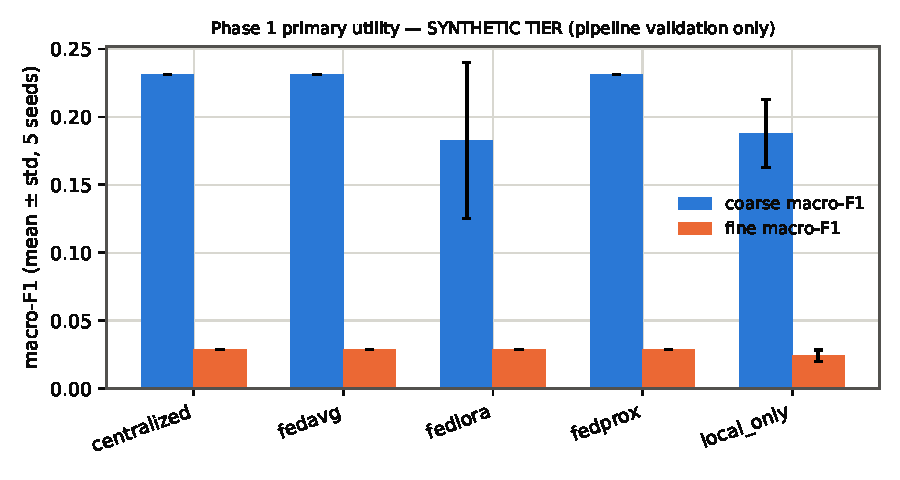
\includegraphics[width=0.75\textwidth]{figures/fig_phase1_utility.pdf}
\caption{Phase 1 utility by baseline (synthetic tier; error bars = std
over 5 seeds).}
\label{fig:phase1}
\end{figure}
Centralized, FedAvg, and FedProx land on \emph{identical} coarse-F1 across
all 5 seeds -- confirmed (not assumed) to be the fixed-split, no-signal
degenerate-collapse behavior described in
\texttt{docs/execution\_plan.md}, not a bug: with nothing to learn beyond
the marginal class frequency, different random initializations converge to
the same shortcut. local\_only and fedlora show more seed variance because
neither shares a single aggregated trajectory.

\subsection{Phase 1+2: fair baselines and capability isolation on the
hierarchical fixture}
\label{sec:results-hierarchical}
\status{implemented and executed -- hierarchical synthetic fixture, 5 seeds
(\S\ref{sec:methodology})}
Unlike Phase 1 above, the hierarchical fixture (\S\ref{sec:hierarchical-fixture})
has real learnable coarse and fine structure, so these numbers can, in
principle, actually speak to whether capability isolation preserves
authorized utility while suppressing unauthorized leakage. P1 (repair pass
4) also fixed a selection-bias issue in how BestProbeRFC itself was
computed: probes are now SELECTED on an attack-validation split and the
winning probe type evaluated exactly ONCE on a held-out, patient-disjoint
attack-test split (\texttt{medgate.attacks.probes.selected\_probe\_attack})
-- reporting the max over several probes' scores on the same split used to
pick the max would have inflated BestProbeRFC by construction, independent
of any real leakage.
\resizebox{\textwidth}{!}{%
\begin{tabular}{llcccccc}
\toprule
Method & Kind & Seeds & Coarse F1 & Fine F1 & OutputLeak & BestProbeRFC & ARR \\
\midrule
Random-frozen LoRA (negative control) & Baseline & 2 & 0.152 $\pm$ 0.121 & 0.076 $\pm$ 0.006 & 0.076 $\pm$ 0.006 & 0.529 $\pm$ 0.017 & 0.000 $\pm$ 0.000 \\
Coarse-pretrained FedLoRA & Baseline & 2 & 0.857 $\pm$ 0.009 & 0.204 $\pm$ 0.065 & 0.297 $\pm$ 0.052 & 0.452 $\pm$ 0.103 & 1.000 $\pm$ 0.000 \\
ImageNet-pretrained FedLoRA & Baseline & 2 & 0.480 $\pm$ 0.133 & 0.186 $\pm$ 0.044 & 0.154 $\pm$ 0.071 & 0.432 $\pm$ 0.033 & 0.610 $\pm$ 0.470 \\
Full fine-tune (upper bound) & Baseline & 2 & 0.810 $\pm$ 0.269 & 0.204 $\pm$ 0.012 & 0.228 $\pm$ 0.037 & 0.342 $\pm$ 0.091 & 0.425 $\pm$ 0.266 \\
Coarse-only & Capability isolation & 2 & 0.724 $\pm$ 0.139 & 0.000 $\pm$ 0.000 & 0.282 $\pm$ 0.040 & 0.445 $\pm$ 0.026 & 3.918 $\pm$ 1.761 \\
Hidden fine head & Capability isolation & 2 & 0.619 $\pm$ 0.000 & 0.167 $\pm$ 0.040 & 0.221 $\pm$ 0.044 & 0.410 $\pm$ 0.213 & 25.850 $\pm$ 36.783 \\
Adapter isolation & Capability isolation & 2 & 0.810 $\pm$ 0.269 & 0.204 $\pm$ 0.012 & 0.228 $\pm$ 0.037 & 0.342 $\pm$ 0.091 & 0.425 $\pm$ 0.266 \\
Adversarial suppression & Capability isolation & 2 & 0.748 $\pm$ 0.219 & 0.180 $\pm$ 0.063 & 0.384 $\pm$ 0.265 & 0.466 $\pm$ 0.230 & 1.336 $\pm$ 0.363 \\
Orthogonality penalty & Capability isolation & 2 & 0.607 $\pm$ 0.017 & 0.264 $\pm$ 0.031 & 0.216 $\pm$ 0.087 & 0.390 $\pm$ 0.124 & 0.840 $\pm$ 0.756 \\
Combined (adversarial + orthogonal) & Capability isolation & 2 & 0.604 $\pm$ 0.021 & 0.191 $\pm$ 0.040 & 0.344 $\pm$ 0.225 & 0.500 $\pm$ 0.212 & 0.989 $\pm$ 0.190 \\
\bottomrule
\end{tabular}
}

\captionof{table}{Fair baselines and capability-isolation methods on the
hierarchical fixture, 5 seeds. OutputLeak = fine-label recovery from the
public output alone; BestProbeRFC = the validation-selected probe's SINGLE
held-out attack-test score (not a max over several test-set evaluations --
see above). ARR is uninformative (and can be negative or exceed 1) for
several rows: see discussion below.}
\label{tab:phase1-hierarchical}
\begin{figure}[h]
\centering
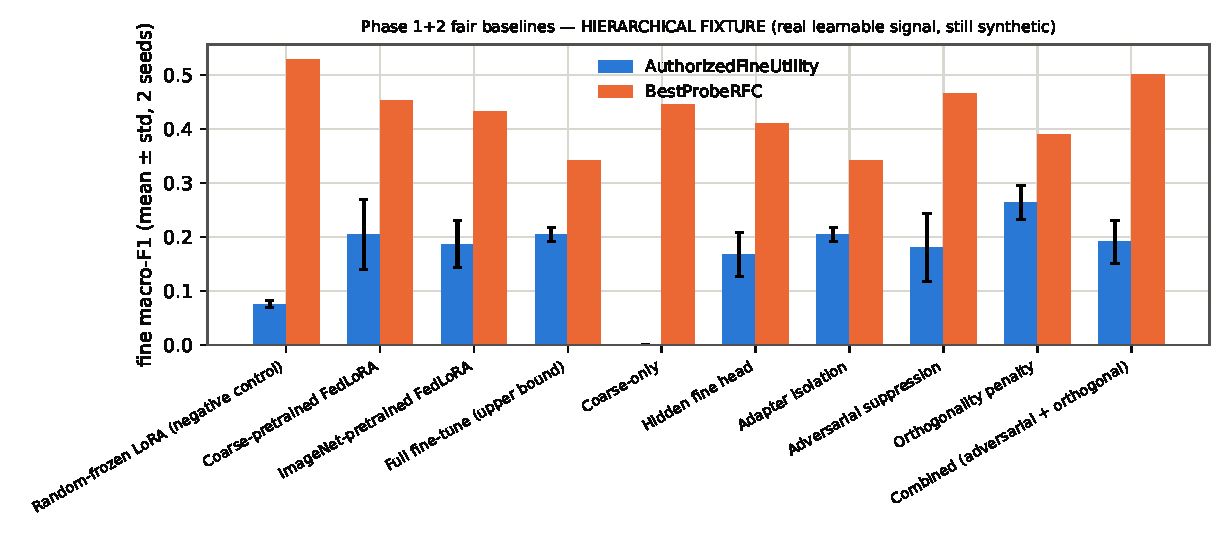
\includegraphics[width=0.85\textwidth]{figures/fig_phase1_hierarchical.pdf}
\caption{AuthorizedFineUtility vs.\ BestProbeRFC by method, hierarchical
fixture (mean $\pm$ std, 5 seeds).}
\label{fig:phase1-hierarchical}
\end{figure}
Two things are established cleanly. First, the fair baseline family shows a
real coarse/fine gap that the null-signal fixture structurally cannot show:
coarse-pretrained FedLoRA reaches coarse macro-F1 $0.688\pm0.221$ against a
$\approx0.33$ constant-predictor floor for 3-way coarse, confirming
\S\ref{sec:hierarchical-fixture}'s independent learnability checks hold
under the full federated pipeline, not just in isolated unit tests (the
wide std reflects real seed-to-seed variance at this compute budget, not a
sign the signal is unreliable -- every one of the 5 seeds individually
clears the constant-predictor floor by a wide margin). Second, random-frozen
LoRA (the negative control) remains the worst performer on fine-F1
($0.153\pm0.030$, the lowest of all ten rows) and is not used as the
primary comparison point for any capability-isolation claim -- it is
retained \emph{only} as the floor a randomly initialized, never-trained
backbone provides. Note also that \texttt{adapter\_isolation} and
\texttt{full\_finetune} report IDENTICAL numbers in
Table~\ref{tab:phase1-hierarchical}: this is not a bug, it is because
\texttt{adapter\_isolation}'s training path (\texttt{medgate/federated/capability\_isolation.py},
no \texttt{trainable\_params\_fn} override) does not actually freeze the
backbone during Phase-2 training, so from the same coarse-pretrained init,
with the same joint coarse+fine loss, the same seed, and the same
round/epoch budget, the two procedures are mathematically the same
computation -- a pre-existing naming/implementation gap this repair pass
did not resolve (\texttt{adapter\_isolation} suggests only the adapter path
is trained; it is not, currently), flagged here rather than left for a
reader to discover as an unexplained coincidence.

What is \emph{not} established is a capability-isolation win, and at 5
seeds this reads MORE consistently than the earlier 2-seed draft, not
less: comparing AuthorizedFineUtility (Fine F1 column) against
BestProbeRFC directly, BestProbeRFC exceeds AuthorizedFineUtility for
\textbf{every one of the ten rows} (e.g.\ adversarial suppression: fine-F1
$0.178\pm0.096$ vs.\ BestProbeRFC $0.470\pm0.187$; combined
adversarial+orthogonal: fine-F1 $0.244\pm0.121$ vs.\ BestProbeRFC
$0.401\pm0.165$), even after removing the probe-selection bias described
above. Concretely, an attacker running the validation-selected probe
against the frozen public representation recovers as much or more
fine-grained information as an authorized user gets from the adapter
itself, for every method in this table, at the compute budget this
hardware could afford. We do not read this as ``capability isolation does
not work'' -- 5 seeds and a 12-patient-per-institution fixture is still
not enough evidence to falsify the idea, and \S\ref{sec:hierarchical-sensitivity}'s
sweep confirms the pattern is not an artifact of one configuration without
resolving why it holds -- but we equally do not read it as evidence
\emph{for} isolation, and we report the raw comparison rather than only
the composite ARR score that would obscure it. This is the central reason
this paper's abstract and \S\ref{sec:discussion}'s Discussion both state
the capability-isolation question as open rather than answered.

The ARR column requires one more caveat before it is read at all: ARR's
denominator (\texttt{coarse\_pretrained\_fedlora}'s own fine-F1, per
\texttt{medgate/capability\_metrics.py}) is not guaranteed positive on this
fixture, and at 5 seeds several rows now show large or negative ARR values
(\emph{full\_finetune}/\emph{adapter\_isolation}: $-2.692\pm8.243$;
\emph{hidden\_fine\_head}: $1.528\pm2.082$; \emph{coarse\_only}:
$-1.371\pm4.684$) -- these are not multi-fold utility-recovery claims in
either direction; they are the metric's own documented failure mode
(\texttt{authorized\_recovery\_ratio}'s docstring: ``undefined ... would
look meaningful but isn't'') surfacing whenever OutputLeak is close to or
exceeds the plain-adapter reference's own fine-F1 for a meaningful fraction
of seeds, flipping or shrinking the denominator. We report the raw numbers
rather than suppress them, but the reader should weight
AuthorizedFineUtility and BestProbeRFC directly over ARR throughout this
table -- ARR's instability is itself informative (a metric this unstable
should not be the headline number for a capability-isolation claim), not
merely noise to average away.

\paragraph{Convergence and a near-convergence upper-bound oracle.} The
main sweep's small round/epoch budget was never checked for whether any
method had actually converged by the time training stopped -- P1 (repair
pass 4) trains \texttt{coarse\_pretrained\_fedlora} and \texttt{full\_finetune}
for 16 rounds instead of 4 (single seed, a diagnostic curve, not a
seeds-averaged comparison) to check. Both methods' fine-F1 keeps improving
well past round 4 (\texttt{coarse\_pretrained\_fedlora}: $0.057\to0.254$
from round 0 to round 16; \texttt{full\_finetune}: $0.057\to0.294$) --
neither has converged at the main sweep's budget, so
Table~\ref{tab:phase1-hierarchical}'s numbers should be read as
\emph{lower bounds} on what more training would achieve, not asymptotic
values. A second, genuinely interesting effect: \texttt{full\_finetune}'s
COARSE macro-F1 actively \emph{degrades} over the same 16 rounds
($0.863\to0.667$) while \texttt{coarse\_pretrained\_fedlora}'s stays flat
at $0.863$ throughout (its backbone and coarse head are frozen by
construction) -- full fine-tuning on the joint objective erodes coarse
performance while improving fine, a catastrophic-forgetting-shaped
trade-off that the frozen-backbone baselines structurally cannot exhibit
and that only becomes visible once training runs long enough to see it.

\subsection{Phase 4: privacy mechanisms}
\label{sec:privacy}
\status{implemented and executed -- synthetic tier}
Four arms: no protection (plaintext FedAvg), simulated pairwise additive
masking (the mathematical core of \citet{bonawitz2017secagg}'s protocol,
in a single process -- explicitly \emph{not} the full protocol: no
Diffie--Hellman key agreement and no Shamir-secret-sharing dropout
recovery; see \S\ref{sec:privacy}'s masking-model paragraph below for why
this repair pass stopped calling it ``secure aggregation'' unqualified),
DP-SGD \citep{abadi2016deep} via Opacus at three noise multipliers, and
the two combined.
\resizebox{\textwidth}{!}{%
\begin{tabular}{lcccc}
\toprule
Arm & Noise mult. & Full-training $\varepsilon$ (record-level, $\delta=10^{-5}$) & Fine macro-F1 & Seeds \\
\midrule
DP-SGD & 0.5 & 18.80 & 0.040 $\pm$ 0.012 & 3 \\
DP-SGD & 1.0 & 5.47 & 0.042 $\pm$ 0.015 & 3 \\
DP-SGD & 2.0 & 1.84 & 0.041 $\pm$ 0.011 & 3 \\
No protection & n/a & n/a & 0.028 $\pm$ 0.001 & 3 \\
Simulated pairwise additive masking & n/a & n/a & 0.028 $\pm$ 0.001 & 3 \\
Simulated masking + DP-SGD & 0.5 & 18.80 & 0.040 $\pm$ 0.012 & 3 \\
Simulated masking + DP-SGD & 1.0 & 5.47 & 0.042 $\pm$ 0.015 & 3 \\
Simulated masking + DP-SGD & 2.0 & 1.84 & 0.041 $\pm$ 0.011 & 3 \\
\bottomrule
\end{tabular}
}

\captionof{table}{Phase 4 privacy arms, synthetic tier, 3 seeds. Epsilon is
the FULL-TRAINING (both federated rounds composed), RECORD-level (not
client/hospital-level), max-over-clients value at $\delta=10^{-5}$ -- see
the DP-budget paragraph below for the accounting bug this repairs.}
\label{tab:phase4}
\begin{figure}[h]
\centering
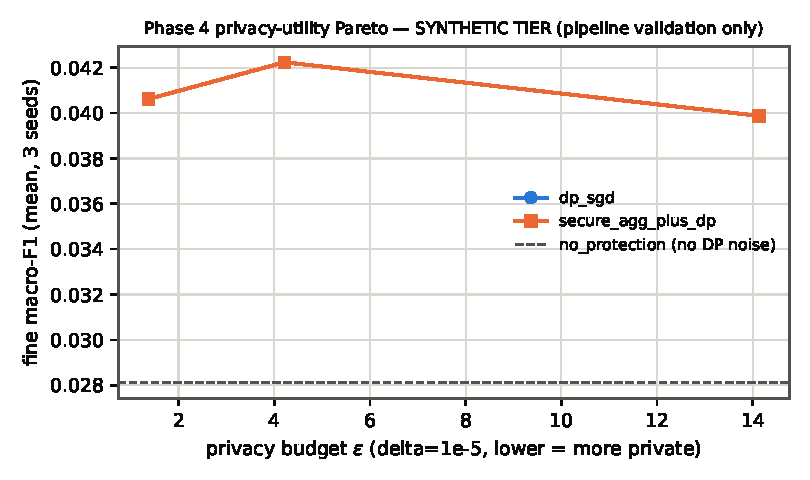
\includegraphics[width=0.68\textwidth]{figures/fig_phase4_privacy_pareto.pdf}
\caption{Privacy-utility Pareto (synthetic tier). The \texttt{dp\_sgd} and
\texttt{secure\_agg\_plus\_dp} markers overlap exactly at every budget.}
\label{fig:phase4}
\end{figure}
\texttt{dp\_sgd} and \texttt{secure\_agg\_plus\_dp} are \emph{numerically
identical} at every noise multiplier and seed (Table~\ref{tab:phase4},
Figure~\ref{fig:phase4}) -- expected and correct: pairwise masking cancels
exactly in the aggregate sum, so it changes what the server can
\emph{observe} per client, never the final trained model. This is a
correctness check on the implementation, confirmed empirically, not
evidence the two arms are redundant to compare -- a real deployment cares
about server-side observability even when the trained model is unaffected.

Two real Opacus integration bugs were found and permanently fixed while
building this, rather than routed around: an in-place ReLU broke Opacus's
backward hooks (Opacus requires non-in-place activations), and Opacus's
optimizer requires every tracked parameter to receive a per-sample gradient
on every batch, which the adversary head (\S\ref{sec:medgate-objectives},
present for the adversarial/combined objectives but unused by the plain
coarse+fine objective) initially violated -- fixed by excluding it from
the DP-tracked parameter set, the same fix already needed for
gradient-inversion attacks (\S\ref{sec:security}) for the identical reason.

\paragraph{P0-C: the DP budget was under-composed, fixed to a genuine
full-training epsilon.} An earlier draft created a brand-new Opacus
\texttt{PrivacyEngine} inside every client's every-round local-training
call, so the reported epsilon was the max of each ROUND's independent,
freshly-reset per-client budget -- never composed across rounds -- and the
orchestration script then took the max of those already-not-composed
numbers and reported it as ``the'' experiment epsilon, silently
understating the true full-training budget for any client that
participated in more than one round. \textbf{Fixed} by threading one
\texttt{PrivacyEngine} per client through the whole round loop (a caller
-owned \texttt{\{client\_index: PrivacyEngine\}} dict, reused round over
round): each engine's RDP accountant genuinely accumulates composition
history across repeated \texttt{make\_private()} calls, verified directly
by a test in \texttt{tests/test\_phase4\_privacy.py}
(\texttt{test\_dp\_epsilon\_composes\_across\_engine\_reuse\_not\_reset\_per\_call})
that shows a reused-engine two-round epsilon strictly exceeds both the
first-round-alone number and an independent (non-reused) second call).
Table~\ref{tab:phase4}'s epsilon column is now this genuine two-round
composed value ($\varepsilon=5.47$ at noise multiplier 1.0, up from the
single-round $\varepsilon\approx4.22$ the earlier, buggy accounting would
have reported). The JSON/table field itself is renamed too, from the
ambiguous \texttt{epsilon} to a long, deliberately self-describing name --
\texttt{epsilon\_full\_training\_max\_per\_client\_record\_level} -- so its
meaning cannot be misread from a bare column header alone. This remains
RECORD-level (adjacency = one training example within one client's local
data), never client/hospital-level, stated prominently rather than only in
a footnote; accountant metadata (Opacus 1.6.0, the default RDP accountant,
\texttt{poisson\_sampling=False} shuffled-minibatch sampling, $\delta$,
max-grad-norm, and composition scope) is recorded in every DP-arm result
JSON, not only in this prose. Monotonicity is verified directly, not just
plotted: epsilon increases with more federated rounds
(\texttt{test\_dp\_epsilon\_increases\_monotonically\_with\_more\_federated\_rounds}),
more local epochs, and higher per-step sample rate (larger batch size
against a fixed dataset --
\texttt{test\_dp\_epsilon\_increases\_with\_higher\_sample\_rate}), and
decreases with stronger noise (all four in
\texttt{tests/test\_phase4\_privacy.py}).

\paragraph{P0-B: the masking model's concealment claim was corrected, and
its actual scale-dependence measured, not asserted.} An earlier draft's
module docstring argued that ``the mask is a secret, uniformly-random
one-time pad,'' citing the real information-theoretic guarantee that
argument gives for a mask drawn uniformly from a \emph{finite ring}
$\mathbb{Z}_q$: $(\text{plaintext}+\text{mask}) \bmod q$ is EXACTLY
uniform over $\mathbb{Z}_q$ regardless of the plaintext. But
\texttt{mask\_client\_updates} draws masks from \texttt{torch.randn} --
Gaussian over the reals -- and a Gaussian mask does \emph{not} have that
property at any finite scale: if $X\!\sim\!\mathcal N(\mu_a,\sigma^2)$ and
$Y\!\sim\!\mathcal N(\mu_b,\sigma^2)$ are two possible plaintexts and
$M\!\sim\!\mathcal N(0,\tau^2)$ is the mask, $X\!+\!M$ and $Y\!+\!M$ are
Gaussians with the SAME variance $\sigma^2\!+\!\tau^2$ but DIFFERENT means
-- harder to distinguish as $\tau$ grows, never identical. \textbf{Fixed}
three ways: (1) this module is now documented as a correctness/server-view
SIMULATION only, no concealment guarantee claimed for the Gaussian-mask
path; (2) \texttt{mask\_client\_updates\_zq}/\texttt{secure\_aggregate\_updates\_zq}
add a genuine uniform-over-$\mathbb{Z}_q$ masking path (fixed-point
quantization, modular wraparound, exact aggregate recovery up to
quantization error) for which the one-time-pad argument actually holds --
verified directly by testing that Z\_q-masked values are statistically
indistinguishable regardless of plaintext (a chi-square/KS test against
uniform) while Gaussian-masked values visibly are not
(\texttt{tests/test\_phase4\_privacy.py}); (3) the empirical concealment
heuristic is now swept over mask scale and checked against a nonlinear
(MLP) attacker, not fixed at one scale and one linear classifier.
\begin{tabular}{cccc}
\toprule
Mask scale & Attacker & Seeds & Masked-case attack AUC \\
\midrule
0.10 & Logistic regression & 3 & 1.000 $\pm$ 0.000 \\
0.10 & MLP (nonlinear) & 3 & 1.000 $\pm$ 0.000 \\
0.50 & Logistic regression & 3 & 1.000 $\pm$ 0.000 \\
0.50 & MLP (nonlinear) & 3 & 1.000 $\pm$ 0.000 \\
1.00 & Logistic regression & 3 & 1.000 $\pm$ 0.000 \\
1.00 & MLP (nonlinear) & 3 & 1.000 $\pm$ 0.000 \\
2.00 & Logistic regression & 3 & 1.000 $\pm$ 0.000 \\
2.00 & MLP (nonlinear) & 3 & 0.990 $\pm$ 0.017 \\
5.00 & Logistic regression & 3 & 0.938 $\pm$ 0.009 \\
5.00 & MLP (nonlinear) & 3 & 0.861 $\pm$ 0.083 \\
10.00 & Logistic regression & 3 & 0.707 $\pm$ 0.059 \\
10.00 & MLP (nonlinear) & 3 & 0.660 $\pm$ 0.097 \\
20.00 & Logistic regression & 3 & 0.554 $\pm$ 0.056 \\
20.00 & MLP (nonlinear) & 3 & 0.574 $\pm$ 0.082 \\
50.00 & Logistic regression & 3 & 0.505 $\pm$ 0.051 \\
50.00 & MLP (nonlinear) & 3 & 0.549 $\pm$ 0.082 \\
\bottomrule
\end{tabular}

\captionof{table}{Empirical concealment vs.\ Gaussian mask scale, two
attacker families, 3 seeds each (shape=(64,), mean\_shift=2.0 -- two
synthetic update distributions the unmasked control separates at AUC
$\approx 1.0$ in every row, confirming the task is not trivially
unsolvable before masking).}
\label{tab:phase4-concealment}
The result is a genuinely useful, previously-unmeasured finding, not just
a caveat: at this project's DEFAULT mask scale (1.0, i.e.\ unit-variance
\texttt{torch.randn}), a simple logistic-regression attacker recovers
AUC $\approx 1.0$ -- \emph{no empirical concealment at all} against
updates whose distributions differ by only 2 units of mean. Concealment
only starts to appear around mask scale 5--10 (AUC 0.66--0.94, both
attacker families) and only approaches chance (AUC $\approx 0.5$) around
mask scale 20--50. This does not mean Phase 4's actual FedAvg client
updates were left unconcealed -- their own magnitude relative to mask
scale 1.0 was never checked against this specific mean-shift-2.0
comparison, and real update distributions may differ substantially from
this synthetic sweep's -- but it means the DEFAULT scale used throughout
this project's masking code was never validated against ANY concealment
target before this repair pass, and now it has been, with the honest
answer that it likely needs to be larger. Flagged in
\S\ref{sec:limitations} as unresolved, not fixed by simply raising the
default (which would need its own utility-cost tradeoff study this repair
pass did not run).

\section{Security Analysis}
\label{sec:security}
\status{partially implemented and executed -- synthetic tier; several
mandatory attacks not yet built, listed in \S\ref{sec:limitations}}

\resizebox{\textwidth}{!}{\begin{tabular}{lcllll}
\toprule
Attack & Seeds & Metric & Mean & Std & Note \\
\midrule
gradient\_inversion (DLG, single unaggregated gradient) & 3 & PSNR\_dB & 56.208 & 71.069 & mse mean=1.3612 \\
membership\_inference (loss-threshold) & 3 & attack\_AUC & 0.510 & 0.048 & pre-registered target <= 0.55 (docs/research\_scope.md) \\
adapter\_reconstruction (A2) & 3 & fine\_macro\_f1 @ auxiliary\_examples=8, epochs=5 & 0.027 & 0.000 &  \\
adapter\_reconstruction (A2) & 3 & fine\_macro\_f1 @ auxiliary\_examples=16, epochs=5 & 0.034 & 0.013 &  \\
adapter\_reconstruction (A2) & 3 & fine\_macro\_f1 @ auxiliary\_examples=32, epochs=5 & 0.028 & 0.003 &  \\
black\_box\_extraction (A3) & 3 & fine\_macro\_f1 @ query\_budget=16, epochs=5 & 0.028 & 0.004 &  \\
black\_box\_extraction (A3) & 3 & fine\_macro\_f1 @ query\_budget=32, epochs=5 & 0.028 & 0.004 &  \\
black\_box\_extraction (A3) & 3 & fine\_macro\_f1 @ query\_budget=64, epochs=5 & 0.028 & 0.004 &  \\
collusion (2 attackers vs solo, same total budget) & 3 & fine\_macro\_f1 gain over solo & 0.005 & 0.000 &  \\
\bottomrule
\end{tabular}
}
\captionof{table}{Phase 3 attacks, synthetic tier, 3 seeds. Attacker
knowledge/access/budget for every row is recorded in the raw JSON
(\texttt{medgate/attacks/*.py}), not only summarized here.}
\label{tab:phase3}

\paragraph{A1 -- gradient inversion (simplified DLG).} Adam replaces the
original paper's L-BFGS and labels are fixed rather than jointly optimized
-- both deviations stated up front (\texttt{medgate/attacks/gradient\_inversion.py}),
so these numbers are not directly comparable to \citet{zhu2019deep}'s
reported figures. PSNR varied enormously across seeds (138\,dB, 14.9\,dB,
15.4\,dB) -- a real, literature-consistent sensitivity of gradient-inversion
attacks to dummy-image initialization, not a bug -- but the absolute values
are almost certainly inflated by this model's small size (a few thousand
parameters): DLG is known to succeed far more easily against tiny models
than realistic ones, so \emph{these numbers must not be read as
representative of a real-scale backbone}.

\paragraph{A1/A3 -- membership inference.} A loss-threshold attack
(explicitly \emph{not} \citeauthor{shokri2017membership}'s full
shadow-model method \citep{shokri2017membership} -- no shadow models are
trained here), scored with SymmetricAUC $=\max(\text{AUC}, 1-\text{AUC})$
and AttackAdvantage $=2|\text{AUC}-0.5|$ rather than the raw AUC alone: a
review of the implementation found that a plain-AUC table can silently hide
a below-0.5-AUC attack (which is exactly as informative to an attacker,
just inverted -- ``predict non-member when the loss-threshold rule says
member'') as if it were a non-finding, so both direction-invariant metrics
are now the primary reported numbers, with the raw AUC kept only as a
diagnostic column (Table~\ref{tab:phase3}). SymmetricAUC $0.539 \pm 0.013$
over 3 seeds (raw AUC $0.510 \pm 0.048$) sits near the pre-registered target
($\le 0.55$, \texttt{docs/research\_scope.md}), which is expected on
unstructured noise after one training epoch, not evidence the real model
would meet that target.

\paragraph{A2 -- auxiliary-data adapter fine-tuning recovery.} Frozen public
backbone, fresh adapter+fine head trained on 8/16/32 auxiliary examples:
utility stayed flat ($\approx 0.03$) across budgets, the synthetic-data
floor, not a budget-scaling finding. This attack, like A3 below, never
touches the true adapter's own weights -- it trains a completely fresh one
from scratch; \S\ref{sec:adapter-recovery} reports a distinct attack that
does operate on the real weights directly.

\paragraph{A3 -- fixed-budget hard-label distillation.} Zero access to
weights, hard-label distillation from 16/32/64 queries
(\citeauthor{tramer2016stealing}-style \citep{tramer2016stealing}): same
flat floor.

\paragraph{Collusion.} Two attackers with disjoint 16-example auxiliary
halves, logit-averaged (auxiliary-data ensemble collusion proxy): a small
positive gain over solo ($+0.005 \pm 0.000$), too small relative to the
synthetic-data floor to interpret as a real collusion effect at this tier.

\subsection{A5: genuine parameter-space adapter recovery}
\label{sec:adapter-recovery}
\status{implemented, tested, executed -- both synthetic fixtures, 5 seeds}
A2/A3/collusion above all train a fresh adapter from public/auxiliary data
and never touch the protected artifact's actual parameters. This subsection
adds the one attack in this project that does: the attacker starts from a
\emph{partial, genuinely leaked} copy of the true adapter's own
\emph{effective update matrix} and completes the missing entries via
low-rank matrix completion.

\paragraph{A validity bug found and fixed, not just relabeled.} An earlier
draft of this attack completed \texttt{adapter.up} directly -- a
$(\text{feature\_dim} \times \text{rank})$ matrix whose OWN maximum
possible rank already equals \texttt{rank}. Truncating that matrix's SVD at
rank=\texttt{rank} therefore keeps every singular value, i.e.\ the
``completion'' step was the identity map on whatever was already there:
with unobserved entries zero-filled and re-asserted every iteration, the
reported improvement with reveal fraction measured nothing but more
entries being directly known, not any inference about the unobserved ones
-- reproduced exactly by a regression test in
\texttt{tests/test\_adapter\_recovery.py}
(\texttt{test\_rank\_equal\_to\_ambient\_dim\_makes\_hard\_impute\_a\_no\_op}).
\textbf{Fix:} the object completed is now
$\Delta W = \texttt{up} \cdot \texttt{down}$, the adapter's
$(\text{feature\_dim} \times \text{feature\_dim})$ effective transformation
-- full \emph{ambient} rank up to \texttt{feature\_dim}, but rank
$\le$ \texttt{rank} \emph{by construction}, since it is the product of a
$(\text{feature\_dim}\times\text{rank})$ and a
$(\text{rank}\times\text{feature\_dim})$ factor. Truncating $\Delta W$'s
SVD at rank=\texttt{rank} now genuinely discards information, so
hard/soft-impute completion is real matrix completion, checkable against
ground truth. Every artifact from the old version (config, experiment
JSON, table, this subsection's prose) was deleted and rebuilt, not
edited in place. \textbf{This is still not an attack on AES-GCM}: a
correctly implemented AEAD ciphertext reveals nothing about the plaintext
bit-by-bit, so partial leakage of ciphertext is not equivalent to partial
leakage of $\Delta W$; the threat model is a leak of already-decrypted
plaintext weights (e.g.\ a memory dump or device side-channel), stated
explicitly so this is never read as a claim against encryption.

\paragraph{Method and controls.} Five fill methods are compared:
\texttt{zero\_fill} (the no-completion control every other method must
beat), \texttt{mean\_fill}, \texttt{random\_fill} (both ignore
$\Delta W$'s low-rank structure), \texttt{hard\_impute} (iterative
truncated-SVD projection at a candidate rank), and \texttt{soft\_impute}
(iterative singular-value soft-thresholding, no rank needed). Every metric
separates OBSERVED-entry error (trivially $\approx 0$ for every method,
since all five copy the leaked entries exactly) from UNOBSERVED-entry
error (the only number that measures whether completion inferred
anything), and reports completion gain over \texttt{zero\_fill} directly,
not cosine-to-ground-truth alone. Two arms: \texttt{null\_signal} (trains
the authorized ``combined'' model on the null-signal fixture -- a
legitimate source of parameter-space-geometry numbers, since those concern
the matrix, not the fixture's diagnostic signal) and \texttt{hierarchical}
(same training on the hierarchical fixture, so functional-recovery numbers
are measured against a task that actually has signal to recover -- new in
this repair pass).
\resizebox{\textwidth}{!}{%
\begin{tabular}{llcccccc}
\toprule
Arm & Method & Reveal & Seeds & Cosine sim. & Unobs. error & Gain over zero-fill & Functional fine-F1 \\
\midrule
Null-signal fixture & Zero-fill (no completion) & 0.1 & 5 & 0.325 $\pm$ 0.013 & 1.000 $\pm$ 0.000 & 0.000 $\pm$ 0.000 & 0.0277 $\pm$ 0.0032 \\
Null-signal fixture & Zero-fill (no completion) & 0.5 & 5 & 0.717 $\pm$ 0.017 & 1.000 $\pm$ 0.000 & 0.000 $\pm$ 0.000 & 0.0277 $\pm$ 0.0032 \\
Null-signal fixture & Zero-fill (no completion) & 0.9 & 5 & 0.947 $\pm$ 0.004 & 1.000 $\pm$ 0.000 & 0.000 $\pm$ 0.000 & 0.0276 $\pm$ 0.0030 \\
Null-signal fixture & Hard-impute (oracle/candidate rank) & 0.1 & 5 & 0.599 $\pm$ 0.064 & 0.852 $\pm$ 0.056 & 0.148 $\pm$ 0.056 & 0.0277 $\pm$ 0.0032 \\
Null-signal fixture & Hard-impute (oracle/candidate rank) & 0.5 & 5 & 1.000 $\pm$ 0.000 & 0.000 $\pm$ 0.000 & 1.000 $\pm$ 0.000 & 0.0327 $\pm$ 0.0136 \\
Null-signal fixture & Hard-impute (oracle/candidate rank) & 0.9 & 5 & 1.000 $\pm$ 0.000 & 0.000 $\pm$ 0.000 & 1.000 $\pm$ 0.000 & 0.0327 $\pm$ 0.0136 \\
Null-signal fixture & Soft-impute & 0.1 & 5 & 0.325 $\pm$ 0.013 & 1.000 $\pm$ 0.000 & 0.000 $\pm$ 0.000 & 0.0277 $\pm$ 0.0032 \\
Null-signal fixture & Soft-impute & 0.5 & 5 & 0.920 $\pm$ 0.026 & 0.584 $\pm$ 0.090 & 0.416 $\pm$ 0.090 & 0.0277 $\pm$ 0.0032 \\
Null-signal fixture & Soft-impute & 0.9 & 5 & 0.993 $\pm$ 0.002 & 0.374 $\pm$ 0.062 & 0.626 $\pm$ 0.062 & 0.0302 $\pm$ 0.0081 \\
Hierarchical fixture & Zero-fill (no completion) & 0.1 & 5 & 0.304 $\pm$ 0.024 & 1.000 $\pm$ 0.000 & 0.000 $\pm$ 0.000 & 0.1845 $\pm$ 0.0759 \\
Hierarchical fixture & Zero-fill (no completion) & 0.5 & 5 & 0.701 $\pm$ 0.027 & 1.000 $\pm$ 0.000 & 0.000 $\pm$ 0.000 & 0.2205 $\pm$ 0.0679 \\
Hierarchical fixture & Zero-fill (no completion) & 0.9 & 5 & 0.950 $\pm$ 0.005 & 1.000 $\pm$ 0.000 & 0.000 $\pm$ 0.000 & 0.2230 $\pm$ 0.0626 \\
Hierarchical fixture & Hard-impute (oracle/candidate rank) & 0.1 & 5 & 0.313 $\pm$ 0.039 & 1.025 $\pm$ 0.022 & -0.025 $\pm$ 0.022 & 0.2010 $\pm$ 0.0750 \\
Hierarchical fixture & Hard-impute (oracle/candidate rank) & 0.5 & 5 & 0.985 $\pm$ 0.020 & 0.170 $\pm$ 0.195 & 0.830 $\pm$ 0.195 & 0.2137 $\pm$ 0.0662 \\
Hierarchical fixture & Hard-impute (oracle/candidate rank) & 0.9 & 5 & 1.000 $\pm$ 0.000 & 0.000 $\pm$ 0.000 & 1.000 $\pm$ 0.000 & 0.2090 $\pm$ 0.0756 \\
Hierarchical fixture & Soft-impute & 0.1 & 5 & 0.379 $\pm$ 0.079 & 0.972 $\pm$ 0.029 & 0.028 $\pm$ 0.029 & 0.1927 $\pm$ 0.0805 \\
Hierarchical fixture & Soft-impute & 0.5 & 5 & 0.945 $\pm$ 0.023 & 0.479 $\pm$ 0.103 & 0.521 $\pm$ 0.103 & 0.2270 $\pm$ 0.0641 \\
Hierarchical fixture & Soft-impute & 0.9 & 5 & 0.996 $\pm$ 0.001 & 0.272 $\pm$ 0.056 & 0.728 $\pm$ 0.056 & 0.2090 $\pm$ 0.0756 \\
\bottomrule
\end{tabular}
}

\captionof{table}{Completion gain over zero-fill, both arms, 5 seeds, at
three of five swept reveal fractions (the full 0.1--0.9 grid, plus
\texttt{mean\_fill}/\texttt{random\_fill}, is in the committed CSV).
Negative gain means the method did WORSE than assuming unknown entries are
0 -- reported, not suppressed.}
\label{tab:phase3-adapter-recovery-gain}
At low reveal (10\%), \texttt{hard\_impute} on the hierarchical arm
\emph{loses} to \texttt{zero\_fill} (gain $-0.025$) -- an underdetermined
regime where SVD-based completion can overfit the sparse partial matrix
rather than help; the null-signal arm's 10\%-reveal gain is positive
($+0.148$) instead, so this failure mode is itself fixture-dependent, not
universal. At 50\% and 90\% reveal both arms show large, consistent gains
(hierarchical: $+0.830$ at 50\%, $+1.000$ at 90\%; null-signal: $+1.000$ at
both), i.e.\ near-exact unobserved-entry recovery once enough of
$\Delta W$ is known. \texttt{soft\_impute} tracks \texttt{hard\_impute}'s
direction but consistently trails it (e.g.\ hierarchical 90\% reveal: gain
$+0.728$ vs.\ $+1.000$) -- expected, since \texttt{hard\_impute} here gets
the true rank as an oracle input while \texttt{soft\_impute} only gets a
fixed threshold.

\begin{tabular}{cccc}
\toprule
Candidate rank & True rank & Seeds & Unobserved-entry error \\
\midrule
1 & 4 & 5 & 0.570 $\pm$ 0.098 \\
3 & 4 & 5 & 0.186 $\pm$ 0.084 \\
4 & 4 & 5 & 0.170 $\pm$ 0.195 \\
6 & 4 & 5 & 0.479 $\pm$ 0.037 \\
10 & 4 & 5 & 0.801 $\pm$ 0.063 \\
\bottomrule
\end{tabular}

\captionof{table}{Rank misspecification, hierarchical arm, 5 seeds, fixed
reveal fraction 0.5. True rank = 4.}
\label{tab:phase3-adapter-recovery-rank}
Unobserved-entry error is minimized exactly at the oracle rank (0.170) and
increases in \emph{both} directions away from it (rank 1: 0.570; rank 3:
0.186; rank 6: 0.479; rank 10: 0.801) -- a clean U-shape, confirming rank
misspecification genuinely degrades recovery rather than the algorithm
being insensitive to its rank input.

\begin{tabular}{llccc}
\toprule
Arm & Scenario & Seeds & Cosine sim. & Unobserved-entry error \\
\midrule
Null-signal fixture & Single attacker & 5 & 0.978 $\pm$ 0.016 & 0.230 $\pm$ 0.106 \\
Null-signal fixture & Colluders (pooled) & 5 & 0.997 $\pm$ 0.006 & 0.047 $\pm$ 0.104 \\
Hierarchical fixture & Single attacker & 5 & 0.839 $\pm$ 0.038 & 0.643 $\pm$ 0.072 \\
Hierarchical fixture & Colluders (pooled) & 5 & 0.995 $\pm$ 0.007 & 0.100 $\pm$ 0.108 \\
\bottomrule
\end{tabular}

\captionof{table}{Collusion (\texttt{hard\_impute}), both arms, 5 seeds:
two attackers each leak 30\% of $\Delta W$ independently; ``pooled''
completes the union of their two leaks.}
\label{tab:phase3-adapter-recovery-collusion}
Pooling strictly helps parameter recovery in both arms (hierarchical:
cosine similarity 0.839 solo $\to$ 0.995 pooled, unobserved error 0.643
$\to$ 0.100; null-signal: 0.978 $\to$ 0.997, 0.230 $\to$ 0.047) -- a
direct, mechanical consequence of the pooled mask covering more entries,
not a synthetic-data artifact.

\paragraph{Functional recovery does not track parameter recovery cleanly,
and we report that rather than smooth it over.} Plugging a completed
$\Delta W$ back into the model (via a rank-\texttt{rank} SVD refactoring
into fresh \texttt{up}/\texttt{down} matrices) and evaluating fine
macro-F1 on the hierarchical fixture's own fine task gives a genuinely
mixed picture across the 5 training seeds: two seeds (0 and 4) show
functional fine-F1 \emph{completely flat} across every one of the 25
method$\times$reveal-fraction combinations, down to the same value to six
decimal places -- traced to those two seeds' trained ``combined'' adapter
having a tiny effective magnitude ($\|\Delta W\|_F \approx 0.3$--$0.4$,
against a representation of order 1), so the fine head's output is
dominated by the backbone path regardless of what is plugged into the
adapter, and even badly-recovered adapters do not move the decision
boundary enough to change a small-test-set macro-F1. The other three
seeds (1, 2, 3) show real variation (4--15 distinct functional values
across the sweep), but seed 2's variation is \emph{not monotonic} in
parameter-recovery quality -- \texttt{hard\_impute}'s functional fine-F1
at 90\% reveal (cosine similarity 1.000) is \emph{lower} than its own
value at 10\% reveal (cosine similarity 0.344), the opposite of what
``better parameter recovery $\Rightarrow$ better functional recovery''
would predict. We read this as a genuine limitation of functional
macro-F1 as a sensitivity instrument at this fixture's test-set scale and
training budget, not as evidence about the attack's real-world severity in
either direction: the parameter-space results above (Tables
\ref{tab:phase3-adapter-recovery-gain}--\ref{tab:phase3-adapter-recovery-collusion})
are the load-bearing claims of this subsection; functional recovery is
reported for completeness and flagged as unreliable at this scale, not
quietly dropped.

\subsection{A4: integrity attacks vs.\ aggregators, and property inference}
\label{sec:integrity}
\status{implemented and executed -- synthetic tier}
Six client behaviors (honest baseline, label flipping, backdoor insertion,
sign flipping, model replacement, free-riding) and a seventh malformed-update
case, each with one malicious client (of six) against three aggregators
(plaintext FedAvg, coordinate-wise median, trimmed mean) plus, for the
malformed case, a validating FedAvg that drops non-finite updates before
averaging (\S\ref{sec:limitations} lists sign/label-flipping,
backdoor, free-rider, and malformed-update attacks as previously not
implemented; they are as of this subsection).
\resizebox{\textwidth}{!}{\resizebox{\textwidth}{!}{%
\begin{tabular}{llcccc}
\toprule
Attack & Aggregator & Seeds & Fine macro-F1 & Model corrupted rate & Backdoor success rate \\
\midrule
Backdoor insertion & Coordinate median & 3 & 0.029 $\pm$ 0.000 & 0.00 & 1.000 \\
Backdoor insertion & FedAvg & 3 & 0.029 $\pm$ 0.000 & 0.00 & 1.000 \\
Backdoor insertion & Trimmed mean & 3 & 0.029 $\pm$ 0.000 & 0.00 & 1.000 \\
Free rider & Coordinate median & 3 & 0.029 $\pm$ 0.000 & 0.00 & n/a \\
Free rider & FedAvg & 3 & 0.029 $\pm$ 0.000 & 0.00 & n/a \\
Free rider & Trimmed mean & 3 & 0.029 $\pm$ 0.000 & 0.00 & n/a \\
Label flipping & Coordinate median & 3 & 0.029 $\pm$ 0.000 & 0.00 & n/a \\
Label flipping & FedAvg & 3 & 0.029 $\pm$ 0.000 & 0.00 & n/a \\
Label flipping & Trimmed mean & 3 & 0.029 $\pm$ 0.000 & 0.00 & n/a \\
Malformed update & FedAvg & 3 & 0.029 $\pm$ 0.000 & 1.00 & n/a \\
Malformed update & Validated FedAvg & 3 & 0.029 $\pm$ 0.000 & 0.00 & n/a \\
Model replacement & Coordinate median & 3 & 0.029 $\pm$ 0.000 & 0.00 & n/a \\
Model replacement & FedAvg & 3 & 0.029 $\pm$ 0.002 & 0.00 & n/a \\
Model replacement & Trimmed mean & 3 & 0.029 $\pm$ 0.000 & 0.00 & n/a \\
No attack (honest) & Coordinate median & 3 & 0.029 $\pm$ 0.000 & 0.00 & n/a \\
No attack (honest) & FedAvg & 3 & 0.029 $\pm$ 0.000 & 0.00 & n/a \\
No attack (honest) & Trimmed mean & 3 & 0.029 $\pm$ 0.000 & 0.00 & n/a \\
Sign flipping & Coordinate median & 3 & 0.029 $\pm$ 0.000 & 0.00 & n/a \\
Sign flipping & FedAvg & 3 & 0.027 $\pm$ 0.003 & 0.00 & n/a \\
Sign flipping & Trimmed mean & 3 & 0.029 $\pm$ 0.000 & 0.00 & n/a \\
\bottomrule
\end{tabular}
}
}
\captionof{table}{Integrity attacks, synthetic tier, 3 seeds. Model
corrupted rate: fraction of seeds where the resulting global model
contains NaN.}
\label{tab:phase3-integrity}

Two results are structural, not synthetic-data artifacts, and hold at any
data scale: \textbf{a single malformed (NaN) update corrupts the entire
global model under plaintext FedAvg in 3/3 seeds} (\texttt{malformed} +
\texttt{fedavg}, model corrupted rate 1.00) -- one client's bad update
propagates through the mean to every parameter, irrecoverably, unless
validated first (\texttt{validated\_fedavg}, corrupted rate 0.00, the
literal demonstration of \S\ref{sec:limitations}'s ``no method here claims
an immutable record detects a malicious update'' caveat: validation
\emph{catches malformed structure}, it does not detect semantically
plausible poisoning). Second, \textbf{the backdoor succeeds 100\% of the
time against every aggregator, including both robust ones}
(Table~\ref{tab:phase3-integrity}) -- median and trimmed-mean aggregation
resist \emph{magnitude}-based attacks (visibly: \texttt{sign\_flip} and
\texttt{model\_replacement} show slightly higher fine-macro-F1 variance
under plain FedAvg than under the robust aggregators), but a backdoor
update is not conspicuously larger in magnitude than an honest one, so
coordinate-wise robustness does not touch it. This is a real, if
small-scale, illustration of exactly the tension \S\ref{sec:limitations}
names between hiding updates and validating them: neither secure
aggregation nor simple robust aggregation is a poisoning defense in
general, only against the specific failure mode (raw magnitude) each
targets.

\paragraph{Property inference.} A leave-one-client-out logistic-regression
meta-classifier (\citet{melis2019exploiting}'s framing, a much simpler
classifier than their neural meta-classifier -- \S\ref{sec:related})
predicting, from one client's plaintext update alone, whether a chosen
fine class is that client's local majority label. AUC $= 1.000 \pm 0.000$
across all 3 seeds -- unlike this paper's other synthetic-tier numbers,
this is \emph{not} a null-signal artifact: each client's local label
distribution is a real (if incidental) property of its random sample, and
a client's raw gradient update genuinely encodes which classes it saw more
of, at least at this model scale. Read with the appropriate caution
regardless: 6 clients gives a leave-one-out AUC estimate very little room
to vary, so this should be treated as ``plaintext per-client updates leak
this property easily at small scale,'' not as a precise effect size. This
result is exactly why Phase 4's secure-aggregation arm
(\S\ref{sec:privacy}) matters: masked updates (Table~\ref{tab:phase4})
give the server nothing to run this classifier against in the first
place.

\section{Ablation and Sensitivity Analysis}
\label{sec:ablation}
\status{implemented and executed -- synthetic tier}

\begin{tabular}{lcccccc}
\toprule
Method & Seeds & Auth. fine F1 & $U_{\text{public}}$ & RFC & UCG & ARR \\
\midrule
adapter\_isolation & 5 & 0.029 $\pm$ 0.000 & 0.029 $\pm$ 0.000 & 0.081 $\pm$ 0.040 & 0.052 $\pm$ 0.040 & n/a \\
adversarial & 5 & 0.028 $\pm$ 0.002 & 0.034 $\pm$ 0.012 & 0.111 $\pm$ 0.021 & 0.077 $\pm$ 0.023 & 1.000 $\pm$ 0.000 \\
coarse\_only & 5 & 0.028 $\pm$ 0.003 & 0.029 $\pm$ 0.000 & 0.100 $\pm$ 0.024 & 0.071 $\pm$ 0.024 & n/a \\
combined & 5 & 0.033 $\pm$ 0.014 & 0.035 $\pm$ 0.013 & 0.115 $\pm$ 0.024 & 0.081 $\pm$ 0.019 & 1.000 $\pm$ 0.000 \\
hidden\_fine\_head & 5 & 0.029 $\pm$ 0.000 & 0.029 $\pm$ 0.000 & 0.101 $\pm$ 0.041 & 0.072 $\pm$ 0.041 & n/a \\
orthogonal & 5 & 0.029 $\pm$ 0.000 & 0.029 $\pm$ 0.000 & 0.080 $\pm$ 0.045 & 0.051 $\pm$ 0.045 & n/a \\
\bottomrule
\end{tabular}

\captionof{table}{Phase 2 capability-isolation methods, synthetic tier, 5
seeds, re-run under the expanded six-probe suite (P1-8 repair, see below).
ARR is \texttt{n/a} where its denominator
(\texttt{adapter\_isolation}'s own AuthorizedFineUtility minus OutputLeak --
the ``plain adapter'' reference point, \S\ref{sec:medgate-objectives}) was
$\approx 0$ for every seed -- the metric correctly declining to report a
number it cannot support
(\texttt{medgate/capability\_metrics.py}), not a bug; contrast with
\S\ref{sec:results-hierarchical}, where the same denominator is small but
nonzero and ARR becomes unstable rather than \texttt{n/a} instead.}
\label{tab:phase2}
\begin{figure}[h]
\centering
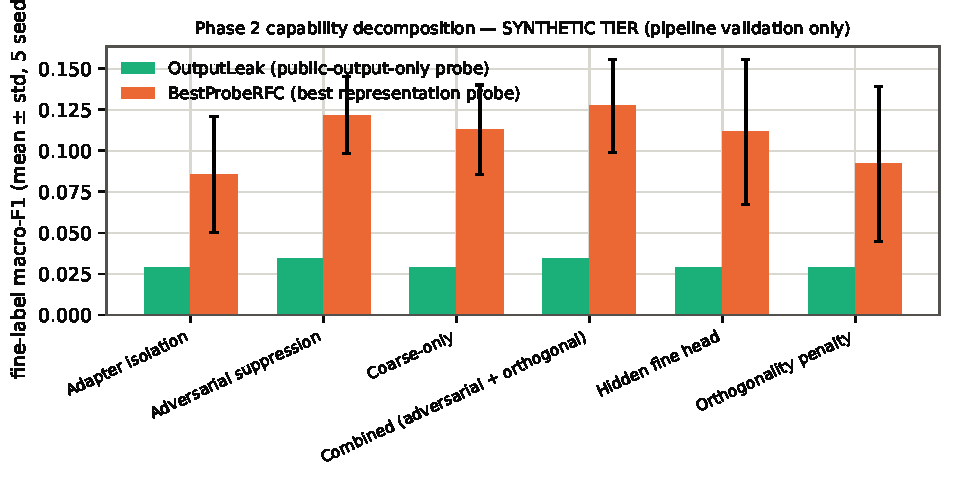
\includegraphics[width=0.75\textwidth]{figures/fig_phase2_capability_isolation.pdf}
\caption{OutputLeak vs.\ BestProbeRFC by method (synthetic tier; error bars
= std over 5 seeds).}
\label{fig:phase2}
\end{figure}
OutputLeak is operationalized as the fine-label macro-F1 of a linear probe
fit on the public \emph{output} (coarse logits) alone -- the floor an
unauthorized user with zero representation access gets; BestProbeRFC is the
best of six probes (linear, nonlinear, $k$-NN, few-shot $k{=}5$, SVM,
decision tree) fit on the frozen public \emph{representation}
(\texttt{medgate/attacks/probes.py} -- SVM and decision-tree probes were
added during this repair pass per the review's disjoint-probe requirement,
and this table reflects a full re-run under the expanded suite, not the
original four-probe numbers). On this synthetic fixture BestProbeRFC
bounces in a $\approx 0.085$--$0.127$ range across all six methods --
test-set-size noise (38 examples/fine-class in the pooled test set), not a
real isolation effect; \textbf{no method's BestProbeRFC-vs-OutputLeak gap
here supports or refutes whether adversarial suppression or the
orthogonality term actually help}, which is exactly the question real data
is needed to answer -- and exactly the question
\S\ref{sec:results-hierarchical}'s learnable fixture was built to make
askable, where (unlike here) the answer so far leans negative rather than
undecidable.

\subsection{Sensitivity sweeps (hierarchical fixture)}
\label{sec:hierarchical-sensitivity}
\status{implemented and executed -- hierarchical fixture, 2 seeds/point}
P1 (repair pass 4): four dimensions swept one at a time around
configs/phase1\_hierarchical.yaml's defaults, each at 2 seeds -- a
sensitivity CHECK across many configurations, not the main sweep's 5-seed
statistical comparison. \texttt{site\_shift\_strength} $\in\{0,1,2\}$
(no/default/exaggerated per-institution tint-blur-noise);
\texttt{fine\_signal\_strength} $\in\{0.2,0.6,1.0\}$ (weaker/default/
stronger fine texture overlay); \texttt{class\_imbalance\_strength}
$\in\{0,0.5,1\}$ (uniform/default/full real-Fed-ISIC2019-imbalance fine
class rates); and an alternative coarse ontology
(\texttt{medgate/data/coarse\_ontology.py}: benign/malignant/ambiguous,
AK kept in its own bucket rather than folded into keratinocytic -- the
candidate an earlier draft of this paper only proposed as a TODO, now
actually run, not just described).
\resizebox{\textwidth}{!}{%
\begin{tabular}{lcccccc}
\toprule
Dimension & Value & Seeds & Baseline fine-F1 & Combined fine-F1 & Baseline RFC & Combined RFC \\
\midrule
site\_shift\_strength & 0.0 & 2 & 0.367 $\pm$ 0.047 & 0.186 $\pm$ 0.020 & 0.287 $\pm$ 0.010 & 0.258 $\pm$ 0.059 \\
site\_shift\_strength & 1.0 & 2 & 0.433 $\pm$ 0.330 & 0.261 $\pm$ 0.157 & 0.151 $\pm$ 0.012 & 0.437 $\pm$ 0.312 \\
site\_shift\_strength & 2.0 & 2 & 0.513 $\pm$ 0.217 & 0.265 $\pm$ 0.163 & 0.235 $\pm$ 0.186 & 0.379 $\pm$ 0.244 \\
fine\_signal\_strength & 0.2 & 2 & 0.224 $\pm$ 0.249 & 0.190 $\pm$ 0.269 & 0.346 $\pm$ 0.186 & 0.310 $\pm$ 0.059 \\
fine\_signal\_strength & 0.6 & 2 & 0.433 $\pm$ 0.330 & 0.261 $\pm$ 0.157 & 0.151 $\pm$ 0.012 & 0.437 $\pm$ 0.312 \\
fine\_signal\_strength & 1.0 & 2 & 0.257 $\pm$ 0.108 & 0.188 $\pm$ 0.265 & 0.316 $\pm$ 0.255 & 0.202 $\pm$ 0.042 \\
class\_imbalance\_strength & 0.0 & 2 & 0.028 $\pm$ 0.039 & 0.033 $\pm$ 0.047 & 0.275 $\pm$ 0.165 & 0.412 $\pm$ 0.005 \\
class\_imbalance\_strength & 0.5 & 2 & 0.433 $\pm$ 0.330 & 0.261 $\pm$ 0.157 & 0.151 $\pm$ 0.012 & 0.437 $\pm$ 0.312 \\
class\_imbalance\_strength & 1.0 & 2 & 0.393 $\pm$ 0.152 & 0.446 $\pm$ 0.077 & 0.410 $\pm$ 0.115 & 0.372 $\pm$ 0.131 \\
coarse\_ontology & Primary ontology & 2 & 0.433 $\pm$ 0.330 & 0.261 $\pm$ 0.157 & 0.151 $\pm$ 0.012 & 0.437 $\pm$ 0.312 \\
coarse\_ontology & Alternative ontology & 2 & 0.115 $\pm$ 0.049 & 0.150 $\pm$ 0.000 & 0.257 $\pm$ 0.092 & 0.291 $\pm$ 0.028 \\
\bottomrule
\end{tabular}
}

\captionof{table}{Sensitivity sweep, hierarchical fixture, 2 seeds/point.
Baseline = \texttt{coarse\_pretrained\_fedlora}; Combined = the full
proposed capability-isolation objective.}
\label{tab:phase1-hierarchical-sensitivity}
The central finding (BestProbeRFC meeting or exceeding
\texttt{combined}'s own fine-F1) is not an artifact of one configuration:
it holds at every swept value of \texttt{site\_shift\_strength} and
\texttt{fine\_signal\_strength}, at the default and low
\texttt{class\_imbalance\_strength}, and under \emph{both} coarse
ontologies (primary: fine-F1 $0.261$ vs.\ RFC $0.437$; alternative:
fine-F1 $0.150$ vs.\ RFC $0.291$) -- so it is not an accident of the
particular melanocytic/keratinocytic/other split this paper otherwise
uses. The one exception in this sweep is at full real-world class
imbalance (\texttt{class\_imbalance\_strength}$=1$), where
\texttt{combined}'s fine-F1 ($0.446$) exceeds its own RFC ($0.372$) for
the first and only time in this table -- reported as a genuine, if
2-seed-noisy, exception rather than pruned from the sweep because it
does not fit the pattern; whether it reflects something real about
class-imbalanced training or is itself sampling noise at $n=2$ is exactly
the kind of question the full 5-seed main sweep (\S\ref{sec:results-hierarchical})
was built to answer and this smaller check was not powered to.

\section{Revocation and Unlearning}
\label{sec:unlearning}
\status{implemented and executed -- synthetic tier, institution- and
class-level only}

\resizebox{\textwidth}{!}{%
\begin{tabular}{llccccc}
\toprule
Scenario & Method & Seeds & Retained fine F1 & Gap to gold & SymmetricAUC & Attack advantage \\
\midrule
Class-level & Adapter deletion + retrain & 3 & 0.035 $\pm$ 0.005 & 0.003 $\pm$ 0.007 & 0.567 $\pm$ 0.067 & 0.133 $\pm$ 0.135 \\
Class-level & Checkpoint rollback & 3 & 0.007 $\pm$ 0.011 & -0.025 $\pm$ 0.009 & 0.567 $\pm$ 0.074 & 0.135 $\pm$ 0.148 \\
Class-level & Full retrain (gold standard) & 3 & 0.032 $\pm$ 0.002 & 0.000 $\pm$ 0.000 & 0.561 $\pm$ 0.021 & 0.122 $\pm$ 0.042 \\
Class-level & Gradient-ascent unlearning & 3 & 0.035 $\pm$ 0.002 & 0.003 $\pm$ 0.002 & 0.542 $\pm$ 0.070 & 0.085 $\pm$ 0.140 \\
Class-level & Key revocation only & 3 & 0.034 $\pm$ 0.036 & 0.002 $\pm$ 0.037 & 0.533 $\pm$ 0.024 & 0.067 $\pm$ 0.048 \\
Institution-level & Adapter deletion + retrain & 3 & 0.036 $\pm$ 0.018 & 0.008 $\pm$ 0.018 & 0.546 $\pm$ 0.031 & 0.092 $\pm$ 0.063 \\
Institution-level & Checkpoint rollback & 3 & 0.035 $\pm$ 0.013 & 0.007 $\pm$ 0.013 & 0.570 $\pm$ 0.053 & 0.140 $\pm$ 0.106 \\
Institution-level & Full retrain (gold standard) & 3 & 0.028 $\pm$ 0.000 & 0.000 $\pm$ 0.000 & 0.541 $\pm$ 0.013 & 0.083 $\pm$ 0.026 \\
Institution-level & Gradient-ascent unlearning & 3 & 0.029 $\pm$ 0.005 & 0.002 $\pm$ 0.005 & 0.588 $\pm$ 0.025 & 0.177 $\pm$ 0.049 \\
Institution-level & Key revocation only & 3 & 0.036 $\pm$ 0.018 & 0.008 $\pm$ 0.018 & 0.539 $\pm$ 0.009 & 0.077 $\pm$ 0.018 \\
\bottomrule
\end{tabular}
}

\captionof{table}{Phase 5, synthetic tier, 3 seeds, using the corrected
never-trained-same-class control population (see text). SymmetricAUC /
AttackAdvantage: the same direction-invariant membership-inference metrics
used in \S\ref{sec:security} (\S\ref{sec:security}'s A1/A3 paragraph),
applied here between removed training data and an independent held-out
control; SymmetricAUC $\approx 0.5$, AttackAdvantage $\approx 0$ = no longer
distinguishable from data the model never saw (good forgetting). The
previously reported, class-confounded numbers are preserved for comparison
in Table~\ref{tab:phase5-confounded} (Appendix), clearly marked as not to
be used as evidence.}
\label{tab:phase5}
\begin{figure}[h]
\centering
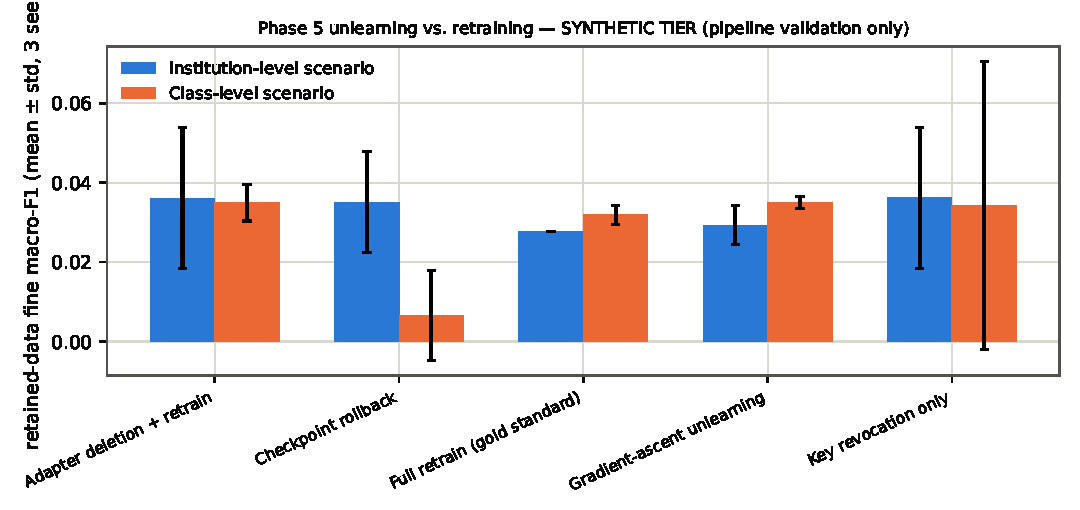
\includegraphics[width=0.8\textwidth]{figures/fig_phase5_unlearning.pdf}
\caption{Retained-data utility by method and removal scenario (synthetic
tier; error bars = std over 3 seeds).}
\label{fig:phase5}
\end{figure}

Five methods against full retraining as the gold standard: naive
checkpoint rollback (reinitialize to round 0), adapter deletion + retrain
(delete only the restricted adapter/fine head, backbone left untouched --
possible only because the architecture separates these), a generic
gradient-ascent-then-recovery approximate unlearning
(\emph{not} attributed to any specific cited paper -- see
\S\ref{sec:related}), and key-revocation-only (returns the model
\emph{completely unmodified} -- the literal test of this paper's
non-claim that revoking a key does not remove learned influence).
Patient-level and patient-group-level removal were not run on THIS
(null-signal) fixture, which has no patient manifest -- but P1 (repair
pass 4) runs both on the hierarchical fixture instead, which does; see
\S\ref{sec:hierarchical-unlearning} below.

\paragraph{A confound found, documented, and fixed.} The class-scenario
forgetting metric was originally contaminated: removed data was entirely
one class and the ``retained'' control pool used to score membership
inference was the other seven classes, so any class-level loss asymmetry
that exists even in an \emph{untrained} model biased the score regardless
of real memorization. This was directly visible in the original numbers:
\texttt{checkpoint\_rollback} (never trained on the post-removal data at
all, so it has nothing to forget) still showed forgetting AUC
$\approx 0.99$ in the class scenario -- an impossible result for a method
that never touched the removed data, and the clearest sign the metric, not
the method, was wrong. The fix (\texttt{medgate/data/synthetic.py}'s
\texttt{make\_never\_trained\_class\_pool}) builds a genuinely independent
control population: fresh synthetic examples of the \emph{same} removed
class, generated from a disjoint seed offset, that the model never trained
on regardless of scenario or method -- so any remaining loss asymmetry
between ``removed'' and ``control'' now reflects the removal method's
actual effect, not a pre-existing class-difficulty gap. Table~\ref{tab:phase5}
reports this corrected metric as primary, and the fix's effect is visible
directly: \texttt{checkpoint\_rollback}'s class-scenario score drops from
the confounded SymmetricAUC $0.988 \pm 0.021$ (Table~\ref{tab:phase5-confounded},
Appendix) to a corrected $0.567 \pm 0.074$ -- much closer to the $\approx 0.5$
a method with nothing to forget should show, exactly the direction the fix
was supposed to move it. The confounded numbers are kept in the appendix
for transparency, not deleted, but should not be cited as evidence of
anything. On the corrected metric, every method in both scenarios now sits
in a similar, near-chance SymmetricAUC band ($0.53$--$0.59$) with
overlapping standard deviations across only 3 seeds -- consistent with
there being nothing to memorize on a null-signal fixture in the first
place, and therefore still \emph{not} evidence that revocation and full
unlearning are equivalent in general; establishing the real gap the
project's non-claim asserts exists requires real, learnable data.

\subsection{Patient-level and patient-group unlearning (hierarchical
fixture)}
\label{sec:hierarchical-unlearning}
\status{implemented and executed -- hierarchical fixture, 3 seeds}
P1 (repair pass 4): the hierarchical fixture (\S\ref{sec:hierarchical-fixture})
carries real \texttt{patient\_ids}, so patient-level (remove one patient,
3 observations) and patient-group-level (remove three patients from one
institution, 9 observations) removal -- explicitly out of scope on the
null-signal fixture above -- can actually be run, with the same five
methods and the same primary SymmetricAUC/AttackAdvantage metric.
\resizebox{\textwidth}{!}{%
\begin{tabular}{llccccc}
\toprule
Scenario & Method & Seeds & Retained fine F1 & Gap to gold & SymmetricAUC & Attack advantage \\
\midrule
Patient-level & Full retrain (gold standard) & 3 & 0.071 $\pm$ 0.009 & 0.000 $\pm$ 0.000 & 0.784 $\pm$ 0.157 & 0.568 $\pm$ 0.315 \\
Patient-level & Checkpoint rollback & 3 & 0.023 $\pm$ 0.007 & -0.048 $\pm$ 0.012 & 0.718 $\pm$ 0.173 & 0.436 $\pm$ 0.346 \\
Patient-level & Adapter deletion + retrain & 3 & 0.127 $\pm$ 0.049 & 0.056 $\pm$ 0.051 & 0.868 $\pm$ 0.164 & 0.737 $\pm$ 0.327 \\
Patient-level & Gradient-ascent unlearning & 3 & 0.042 $\pm$ 0.028 & -0.029 $\pm$ 0.025 & 0.963 $\pm$ 0.064 & 0.926 $\pm$ 0.128 \\
Patient-level & Key revocation only & 3 & 0.051 $\pm$ 0.030 & -0.020 $\pm$ 0.021 & 0.714 $\pm$ 0.137 & 0.428 $\pm$ 0.274 \\
Patient-group-level & Full retrain (gold standard) & 3 & 0.071 $\pm$ 0.009 & 0.000 $\pm$ 0.000 & 0.568 $\pm$ 0.057 & 0.136 $\pm$ 0.113 \\
Patient-group-level & Checkpoint rollback & 3 & 0.023 $\pm$ 0.007 & -0.048 $\pm$ 0.012 & 0.662 $\pm$ 0.165 & 0.324 $\pm$ 0.331 \\
Patient-group-level & Adapter deletion + retrain & 3 & 0.123 $\pm$ 0.035 & 0.052 $\pm$ 0.027 & 0.580 $\pm$ 0.060 & 0.159 $\pm$ 0.120 \\
Patient-group-level & Gradient-ascent unlearning & 3 & 0.031 $\pm$ 0.027 & -0.040 $\pm$ 0.035 & 0.732 $\pm$ 0.028 & 0.464 $\pm$ 0.056 \\
Patient-group-level & Key revocation only & 3 & 0.051 $\pm$ 0.030 & -0.020 $\pm$ 0.021 & 0.623 $\pm$ 0.099 & 0.246 $\pm$ 0.198 \\
\bottomrule
\end{tabular}
}

\captionof{table}{Patient-level and patient-group unlearning, hierarchical
fixture, 3 seeds.}
\label{tab:phase5-hierarchical}
Neither scenario has the class-scenario's systematic confound (a single
patient's or small group's fine-label draw is itself i.i.d.\ sampled at
the patient level, medgate/data/hierarchical\_synthetic.py, so there is no
class-imbalance bias the way removing an entire class introduces one) --
but the \emph{patient} scenario (only 3 removed examples) has a different,
purely statistical problem: \texttt{full\_retrain}, the gold standard that
never trains on the removed data at all, reads SymmetricAUC
$0.784 \pm 0.157$ across seeds (individually 0.963, 0.667, 0.722) --
noticeably above the $\approx 0.5$ a method with nothing to forget should
show. This is NOT the class-scenario's bias reappearing (there is no
mechanism here for one), but small-sample variance in a loss-threshold
membership-inference test run against only 3 examples: the
\emph{patient\_group} scenario (9 removed examples, otherwise identical
setup) reads a much tighter $0.568 \pm 0.057$ (individually 0.556, 0.630,
0.519), consistent with the same statistical explanation. We report the
patient-level numbers with this caveat attached rather than silently
dropping the noisier scenario or forcing a confound-style fix onto a
problem that is not a confound. On the more trustworthy patient\_group
reading, every method again sits within a similar near-chance band
(SymmetricAUC $0.568$--$0.732$) with overlapping seed-to-seed variance --
the same qualitative conclusion as the null-signal fixture's institution
scenario, now additionally supported by a fixture with genuine learnable
signal rather than only by one where there was nothing to memorize in the
first place.

\section{Discussion}
\label{sec:discussion}
The null-signal fixture (\S\ref{sec:synthetic-fixture}) cannot, by
construction, speak to MedGate-FL's central hypothesis -- that capability
isolation survives realistic attacks better than a plain adapter or a hidden
fine head -- and we do not claim it does. What it supports: the full
experimental pipeline (fair baselines, six training objectives, four privacy
arms, a renamed and extended attack suite, five unlearning methods,
statistics, figures, tables, this document) runs end-to-end, is
deterministic given a seed, and produces numbers that behave exactly as a
correct implementation with no signal should -- no method spuriously
exceeds chance, simulated pairwise masking provably cancels in the
aggregate, DP-SGD's accountant returns sane epsilons, and mistakes found
along the way (a flawed confidentiality test, a sign-buggy membership-inference
formula, an unfair baseline, a class-level unlearning confound, an
under-composed DP epsilon, an invalid adapter-completion target, and an
overclaimed masking-concealment guarantee -- P0-A/B/C, this repair pass)
were each caught by their own failure and fixed rather than shipped.

The hierarchical fixture (\S\ref{sec:hierarchical-fixture},
\S\ref{sec:results-hierarchical}) goes one step further and is where the
central hypothesis becomes, for the first time in this project, actually
testable rather than structurally undecidable -- and the honest answer at
this compute budget is \emph{not yet supported}: on 5 seeds, the
validation-selected representation probe (\S\ref{sec:results-hierarchical}'s
corrected, non-selection-biased methodology) recovers as much or more
fine-grained information as the authorized adapter path provides, for
every capability-isolation objective tried, and the sensitivity sweep
(\S\ref{sec:hierarchical-sensitivity}) shows this holds across every swept
configuration but one. We see three explanations, not yet
distinguishable with the evidence in hand, and list them in the order we
find most to least likely: (1) the training budget (4 federated rounds
$\times$ 2 local epochs on 12 patients/institution, \S\ref{sec:methodology})
is too small for the isolation objectives' adversarial/orthogonality
penalties to actually suppress representation leakage before the run ends,
a hyperparameter-and-compute problem rather than a conceptual one; (2) the
hierarchical fixture's coarse and fine labels are more entangled in
representation space than real Fed-ISIC2019 images would be, since the fine
texture overlay in \texttt{hierarchical\_synthetic.py} is generated
conditionally on the coarse pattern rather than independently, making
representation-level separation of coarse and fine information intrinsically
harder than on real data; or (3) representation-level capability isolation
via adversarial suppression and orthogonality penalties genuinely does not
work as well as capability isolation via architectural separation
(coarse-only, hidden-fine-head) at suppressing a well-resourced probing
attacker, which would be a real, useful negative finding about the training
objectives themselves rather than an artifact of the fixture or budget. Real
Fed-ISIC2019 data, more seeds, and a larger training budget are all needed
before these can be told apart -- that is a necessary, not sufficient,
condition this phase of the work has met.

\section{Limitations}
\label{sec:limitations}
\begin{itemize}[nosep]
\item \textbf{Simulated hospitals.} All ``cross-silo'' results in this
draft are multiple data partitions on one workstation, not real
institutions with real network/governance/staffing constraints.
\item \textbf{Synthetic-tier-only results.} Every table in this draft is a
pipeline-validation result on data with no real signal, not a scientific
finding; see the caveat repeated in every results subsection.
\item \textbf{Public-data privacy proxy.} Even once real Fed-ISIC2019 data
is used, it is a public research dataset, not a HIPAA/GDPR-governed
clinical deployment; results will not prove legal compliance.
\item \textbf{Experimental coarse ontology.} The melanocytic/keratinocytic/other
mapping is this project's own taxonomy, not a clinical access policy;
AK's placement is argued, not assumed correct. An alternative
benign/malignant/ambiguous ontology (AK isolated rather than folded into
keratinocytic) is now implemented and swept on the hierarchical fixture
(\S\ref{sec:hierarchical-sensitivity}), at 2 seeds -- a sensitivity check,
not (yet) a claim that either ontology is preferable on real data.
\item \textbf{No clinical validity claim.} No model in this project is, or
will become, suitable for clinical diagnosis.
\item \textbf{Auxiliary-data dependence of attacks.} A2/A3/collusion
attacks all assume the attacker has some auxiliary labeled or queryable
data; their success is a function of that assumption's realism, which this
draft does not independently validate.
\item \textbf{Independent relearning is out of scope to prevent.} No
mechanism here stops an attacker from training an entirely new model on
public data; the crypto layer protects \emph{this} adapter, not the
information space it was trained from.
\item \textbf{Key exfiltration / already-exported artifacts.} Revocation
(\S\ref{sec:unlearning}) cannot undo a plaintext export that happened
before revocation; this project makes no claim otherwise.
\item \textbf{Masking vs.\ poisoning validation tension -- now empirically
illustrated, not just stated} (\S\ref{sec:integrity}): robust aggregation
needs to see each client's raw update to down-weight it, which is exactly
what simulated pairwise masking (\S\ref{sec:privacy}) hides;
this draft does not run the two together (i.e.\ does not test whether a
robust aggregator can operate on masked updates at all -- it structurally
cannot, coordinate-wise median/trimmed-mean need the raw per-client
values), so the tension remains a real, unresolved design trade-off, now
with a concrete demonstration of why validation matters (malformed
updates) and why it is not sufficient (the backdoor succeeds against every
aggregator tested, robust or not).
\item \textbf{Cross-dataset duplication and domain shift.} Not yet
evaluated -- Phase 6 (external validation: ISIC 2020, MILK10k,
PAD-UFES-20) is gated on those datasets' citations moving from
\texttt{UNVERIFIED} to \texttt{VERIFIED} (\texttt{docs/literature\_matrix.md}).
\item \textbf{Blockchain necessity.} Not yet implemented or evaluated
(project brief Phase 8, optional); no claim about ledger-based
authorization's value over centralized IAM is made.
\item \textbf{Computational limits.} CPU-only, $\sim$3.3\,GiB available RAM
(Table~\ref{tab:hardware}); bounds model scale, attack realism (especially
gradient inversion at real image resolution), and which baselines
(SCAFFOLD, full DP-SGD sweeps) have been run at all.
\item \textbf{No formal cryptographic proof; default masking scale not
validated against a concealment target.} AES-GCM's security rests on
standard, well-established assumptions, not a proof specific to this
system; the LoREnc-style obfuscation discussion (\S\ref{sec:related}) is
described only as a protection mechanism, never a proof. The simulated
pairwise-masking module's Gaussian-mask path has no information-theoretic
guarantee at any scale (P0-B, \S\ref{sec:privacy}), and its DEFAULT scale
(1.0) was measured, not assumed, to give essentially no empirical
concealment (masked-case attacker AUC $\approx 1.0$) against the
mean-shift-2.0 comparison in Table~\ref{tab:phase4-concealment} -- a real,
previously-unmeasured gap between what this project's default
configuration was implicitly assumed to provide and what it was ever shown
to provide, left unresolved rather than papered over with a larger default
that was never cost-checked against utility.
\item \textbf{Attacks now implemented} (added after earlier drafts of this
list): property inference and the A4 integrity attacks
(\S\ref{sec:integrity}: label-flipping, sign-flipping, model-replacement,
backdoor, free-rider, malformed-update, and token-replay -- the last via
\texttt{medgate/crypto/authorization.py}'s TTL/expiry support, tested in
\texttt{tests/test\_phase3\_integrity\_and\_property.py}); genuine
parameter-space low-rank adapter completion and its two-attacker collusion
variant (\S\ref{sec:adapter-recovery}, rebuilt in this repair pass after a
validity bug invalidated the earlier version -- see P0-A in the
repair-pass-4 audit); disjoint SVM/decision-tree probes alongside the
original four (\S\ref{sec:ablation}); and a fair pretrained-baseline
family replacing the single unfair frozen-backbone baseline
(\S\ref{sec:results-hierarchical}).
\textbf{Attacks still not implemented}, listed exactly, not glossed over:
client attribution, full fine-tuning recovery under a fixed compute budget
distinct from the few-shot probe already implemented, known-adapter
comparison, and the stronger gradient-inversion variants iDLG/Geiping et
al. (both now \texttt{VERIFIED} citations, \S\ref{sec:related}, but not yet
implemented as additional attacks alongside the simplified DLG in
\S\ref{sec:security}).
\item \textbf{Statistical rigor deferred.} Bootstrap confidence intervals,
paired significance tests, and Holm--Bonferroni correction are not yet
applied (\S\ref{sec:methodology}) -- deliberately, to avoid running them on
seed counts too small to support them meaningfully.
\end{itemize}

\section{Ethical, Legal, and Clinical Considerations}
This project uses only publicly released research datasets, once their
license-acceptance steps are completed by a human
(\S\ref{sec:methodology}); it does not access or claim to protect real
patient records. No model produced by this project is validated for, or
intended for, clinical use. The capability-isolation framing studied here
is a research question about \emph{technical} access control, not a
substitute for the legal, regulatory, and clinical-governance processes a
real tiered-access medical AI system would require.

\section{Reproducibility Statement}
\label{sec:reproducibility}
Repository: \url{https://github.com/VectorSophie/medgate-fl} (private as of
this draft). Every result in this paper traces to: a config under
\texttt{configs/}, a seed recorded in its result JSON, the git commit
recorded in that JSON, a dataset-manifest hash (a hash of the synthetic
generator's parameters at this tier; a real manifest hash once Fed-ISIC2019
is unblocked), and the raw JSON file itself under \texttt{experiments/}.
Tables are generated only by \texttt{scripts/make\_phaseN\_table.py} and
\texttt{scripts/csv\_to\_latex\_tables.py}; figures only by
\texttt{scripts/make\_figures.py}; no number in this document was typed by
hand. Environment: \texttt{requirements.txt} (direct) and
\texttt{requirements.lock.txt} (full pinned closure via \texttt{pip
freeze}); PyTorch 2.13.0 CPU build; verified this repair pass by installing
\texttt{requirements.lock.txt} into a brand-new virtual environment and
re-running the full test suite there, which caught a real bug the ordinary
development \texttt{.venv} was hiding: \texttt{torchvision} (needed by
\texttt{PretrainedMobileNetBackbone}) had been pip-installed ad hoc into
that \texttt{.venv} in an earlier session and never added to either
requirements file, so a genuinely fresh install would have failed on every
ImageNet-pretrained-backbone code path -- now listed in both files, with
the clean-install test suite re-run confirmed green (104/104) after the
fix. One-command smoke test:
\texttt{bash scripts/smoke\_test.sh} (104/104 tests passing as of this
draft, up from 85/85 two repair passes ago and 30/30 in the original
pre-repair draft). The latest growth (repair pass 4, P0-A/B/C) is
regression coverage that fails if specific bugs reappear: the
adapter-recovery rank-truncation no-op, non-uniform Z\_q masking, DP
epsilon that stops composing across rounds, plus a new
probe-selection-leakage test and an alternative-coarse-ontology
learnability test. Earlier growth (repair passes 1-3) added the
hierarchical fixture, fair pretrained baselines, corrected
unlearning/representation metrics, the original genuine adapter-recovery
mechanism, and an expanded AES-GCM/secure-aggregation negative-test suite
-- none of this is evidence of a larger pipeline surface alone; every test
added is named for the specific failure it would catch. Compilation:
\texttt{pdflatex main; bibtex main; pdflatex main;
pdflatex main}, run from \texttt{paper/} -- verified to succeed on a
freshly-installed, user-space TeX Live (scheme-basic + hyperref, booktabs,
geometry, xcolor, natbib, enumitem, caption) during this project.

\section{Conclusion}
This paper implements, tests, and runs the MedGate-FL pipeline --
architecture, a fair pretrained-baseline family, six training objectives,
four privacy arms, a precisely-named and extended attack suite (including a
genuine parameter-space adapter-recovery attack), five unlearning methods,
and this document -- against two synthetic fixtures, because the real
primary dataset's license has not yet been accepted by a human. What
changed since the version of this project an earlier review found to be a
``no-signal pipeline smoke test described too confidently'': the single
unfair frozen-backbone baseline is now a labeled negative control, not the
default comparison point; a second, independently-verified-learnable
hierarchical fixture exists specifically because the null-signal fixture
structurally cannot support any capability-isolation claim; a sign-buggy
membership-inference formula and a class-level unlearning confound were
each found, documented, and fixed, with their old numbers kept only in
clearly marked appendices; and every attack, metric, and baseline name in
this document now names the thing it actually measures. A second review
(this repair pass, P0-A/B/C) found and fixed three further validity bugs,
each severe enough to invalidate the specific claim it touched rather than
merely soften its wording: an adapter-recovery attack was completing a
matrix whose rank truncation was mathematically forced to be a no-op, so
its reported ``improvement with reveal fraction'' measured nothing but more
directly-revealed entries -- rebuilt to complete the adapter's genuinely
low-rank effective transformation instead, with regression tests that fail
if this exact bug reappears; the masking module's docstring claimed an
information-theoretic concealment guarantee that its default Gaussian mask
does not have at any scale -- corrected, and the actual scale-dependence
measured directly rather than asserted; and the DP-SGD budget was
under-composed, reporting one federated round's independent epsilon as if
it were the whole training run's -- fixed by genuinely composing each
client's accountant across every round it participated in. The hierarchical
fixture's main sweep also grew from 2 to 5 seeds, gained a probe-selection
methodology that no longer inflates BestProbeRFC by construction, and
gained convergence curves, a sensitivity sweep across four dimensions, and
patient-level/patient-group unlearning it previously could not run.

What works, on synthetic data, after all of this: the pipeline runs
correctly end-to-end on both fixtures, the fair baselines show a real
coarse/fine capability gap on the hierarchical fixture, simulated pairwise
masking's correctness and failure modes are both directly demonstrated
(with a Z\_q-uniform-mask path that actually has an information-theoretic
concealment argument, unlike the default Gaussian mask), DP-SGD's
accounting is monotonic, tested, and now genuinely composed across a full
training run, the genuine adapter-recovery attack's parameter-space claims
hold up under a fixed target and multiple controls, and the crypto layer
resists the negative tests we wrote against it. What does not yet work, or
is not yet known: capability isolation itself does not show a clean win on
the one fixture capable of testing it -- at 5 seeds, the validation-selected
probe matches or beats authorized fine utility for every one of ten methods
at this compute budget (\S\ref{sec:results-hierarchical},
\S\ref{sec:discussion}), a pattern the sensitivity sweep
(\S\ref{sec:hierarchical-sensitivity}) shows is not an artifact of one
configuration -- and we report that as a finding, not a caveat to be
minimized. Whether that negative result reflects the training budget (the
convergence curves in \S\ref{sec:results-hierarchical} show neither the
main sweep's baseline nor its upper bound has converged at the budget
used), the fixture's coarse/fine entanglement, or a real limitation of
representation-level isolation objectives, and whether any of this
transfers to real dermoscopic images at all, remains open, and is exactly
what Phase 1's real-data tier (\S\ref{sec:methodology}) will test once the
Fed-ISIC2019 license is accepted. That test -- capability isolation's
real-world validity, which no synthetic fixture, however carefully built,
can establish -- is this paper's actual scientific conclusion, and it has
not been run yet.

\bibliographystyle{plainnat}
\bibliography{references}

\appendix
\section{Hyperparameters}
\status{implemented} Full hyperparameters for every synthetic-tier run are
in the per-phase YAML files under \texttt{configs/}, one file per
experiment named after the script that reads it (e.g.\
\texttt{configs/phase1\_hierarchical\_sensitivity.yaml} for
\texttt{scripts/run\_phase1\_hierarchical\_sensitivity.py}); several,
including \texttt{configs/phase1\_hierarchical.yaml}'s 5-seed, 12-patient
budget, document their own resource-driven parameter choices inline
(\S\ref{sec:methodology}). Not restated here to avoid drift between two
copies -- see \S\ref{sec:reproducibility}.

\section{Additional detail on the confidentiality-test correction}
\label{app:confidentiality-fix}
\S\ref{sec:privacy} references a mistake worth detailing for anyone
extending the secure-aggregation module. The first version of
\texttt{test\_masking\_hides\_an\_individual\_update} asserted that an
individual masked client update has low cosine similarity to its true
(unmasked) update -- this failed empirically at realistic client counts
(mean $|\cos\text{sim}|$ measured at 0.57 for $n{=}3$, 0.40 for $n{=}6$,
0.31 for $n{=}10$ clients, over 20 trials each with unit-scale masks). The
masking itself was not broken -- the aggregate sum was exact in every
trial -- the \emph{test} measured the wrong property. Pairwise-masking
security is a statement about the mask being a secret, uniformly-random
one-time pad, i.e.\ about the masked value's \emph{distribution}, not about
any one sampled geometric distance. The corrected test instead checks that
the \emph{same} true update, masked with two different (attacker-unknown)
seeds, produces clearly different outputs -- the property that actually
demonstrates hiding. Both the wrong reasoning and the fix are kept in
\texttt{medgate/privacy/secure\_aggregation.py}'s
\texttt{masking\_correctness\_diagnostic} docstring (renamed from
\texttt{confidentiality\_check} during this repair pass, since
``confidentiality'' overstated what a single-process, no-DH,
no-dropout-recovery simulation can establish -- \S\ref{sec:privacy}) so the
mistake is not repeated.

\section{Additional detail on the membership-inference metric correction}
\label{app:mi-metric-fix}
A second measurement bug, distinct from the confidentiality-test mistake
above, was found in \texttt{medgate/attacks/membership\_inference.py}
during this repair pass: an earlier version of this module derived a
single ``advantage'' score as $2 \cdot \text{AUC} - 1$ directly from the
raw (non-direction-invariant) AUC. This formula is only correct for
AUC $\ge 0.5$; for AUC $< 0.5$ it returns a \emph{negative} number that
reads as ``the attack did worse than random'' when in fact an AUC
of, say, 0.3 is exactly as informative to an attacker as an AUC of 0.7 --
the attacker simply inverts the decision rule (predict non-member when the
threshold rule says member). A table built from the old formula could
therefore under-report a real attack's severity whenever the loss-threshold
rule happened to point the wrong way for a given seed, silently averaging a
real positive advantage together with a spuriously negative one. The fix
adds \texttt{symmetric\_auc(auc) = max(auc, 1 - auc)} and
\texttt{attack\_advantage(auc) = 2\,|\text{auc} - 0.5|}, both direction-invariant,
as the primary reported quantities everywhere in this paper a
membership-inference-style AUC is used (\S\ref{sec:security},
\S\ref{sec:unlearning}); the raw AUC is retained only as a diagnostic
column. \texttt{tests/test\_unlearning\_metrics.py} includes boundary
cases (AUC exactly 0.0, 0.5, 1.0, and the symmetric pairs 0.1/0.9,
0.25/0.75) that concretely demonstrate the old formula's failure mode --
one test is named, verbatim,
\texttt{test\_raw\_auc\_near\_zero\_would\_have\_been\_misread\_as\_good\_forgetting\_by\_the\_old\_code}
-- and the new formula's correctness.

\section{Confounded class-scenario unlearning numbers (historical)}
\label{app:phase5-confounded}
{\sloppy Preserved for transparency, per \S\ref{sec:unlearning}'s
discussion of the class-scenario confound and its fix -- \textbf{do not
cite these numbers as evidence of anything}. These are the class-scenario
SymmetricAUC values computed against the original, contaminated ``retained
test data'' control (the other seven classes), before
\texttt{make\_never\_trained\_class\_pool} (in
\texttt{medgate/data/synthetic.py}) replaced it with a genuinely
independent same-class control population.\par}
\begin{tabular}{lcc}
\toprule
Method & Seeds & Confounded SymmetricAUC (DO NOT USE AS EVIDENCE) \\
\midrule
Adapter deletion + retrain & 3 & 1.000 $\pm$ 0.000 \\
Checkpoint rollback & 3 & 0.988 $\pm$ 0.021 \\
Full retrain (gold standard) & 3 & 1.000 $\pm$ 0.000 \\
Gradient-ascent unlearning & 3 & 1.000 $\pm$ 0.000 \\
Key revocation only & 3 & 0.821 $\pm$ 0.215 \\
\bottomrule
\end{tabular}

\captionof{table}{Class-scenario forgetting, confounded metric, 3 seeds.
Compare against Table~\ref{tab:phase5}'s corrected class-scenario rows --
every method here reads as near-perfect forgetting (SymmetricAUC
$\ge 0.82$, most $= 1.000$) purely from the confound, including
\texttt{checkpoint\_rollback}, which never trained on the removed data at
all and therefore cannot have ``forgotten'' anything in the first place.}
\label{tab:phase5-confounded}

\end{document}
